% All lines that begin with an '%' are comments and won't be displayed in the resulting document1main-branch222

% \documentclass{...} specifies the class of the document. The most common ones are 'book', 'report', 'article' and 'letter'
\documentclass{article}

% Allow the usage of umlauts and other non-ASCII characters
\usepackage[utf8]{inputenc}
% Allow the usage of graphics (.jpg, .png, etc.) in the document
\usepackage{graphicx}
% Allow the change of line spacing
\usepackage{setspace}

% Set line spacing to 1.5xxxneu
\onehalfspacing

% Start the document
\begin{document}

% Show the titlepage (see in 'Documents' below: titlepage.tex)
% Begin a new titlepage. Titlepages have special settings like the absence of page numbers.222
\begin{titlepage}

% Set the text of the page to right-aligned until \end{flushright}
\begin{flushright}

% Set the space between right page border and text to 2.5cm
\rightskip=-2.5cm

% Show an image at this position

\includegraphics[width=50mm]{logo_dark.png}

% Skip a little space
\bigskip
\bigskip
\bigskip
\bigskip

% Create a title for the document and write it in bold font
\LARGE{\textbf{Brief LaTeX Tutorial}}
% Again, do a line break
\linebreak
% Create a subtitle
\large{For LaTeX Beginners}

% Skip some space
\bigskip
\bigskip
\bigskip
\bigskip
\bigskip

% Write in very large letters
\LARGE{verbosus.com}
% Do a line break right after the \LARGE{...} text
\linebreak
% Write in large letters
\large{Free webservices and apps}

% Skip some space
\bigskip
\bigskip
\bigskip
\bigskip
\bigskip
\bigskip

\large{Documentation}

% Skip some space
\bigskip

\normalsize{Vienna, \the\month}

% Skip some space
\bigskip
\bigskip
\bigskip
\bigskip
\bigskip
\bigskip
\bigskip
\bigskip
\bigskip
\bigskip
\bigskip
\bigskip
\bigskip

% Provide some author information
\normalsize{Author:}
\linebreak
\large{Daniel Kuster, MSc}

% End right-alignment at this point
\end{flushright}
% End the title page
\end{titlepage}


% Create a new 1st level heading
\section{First level}

This is the text of the first chapter. If you want to create a subchapter then simply do \textbf{\textbackslash subsection\{Title of first subchapter\}}. If you want to move on to the next chapter then do \textbf{\textbackslash section\{Title of second chapter\}}.

% Create a new 2nd level heading
\subsection{Second level}

Here comes the text of the subsection of the first chapter. Now let's try to insert an image. Currently there exists one image with the name "leaves.jpg" which will be displayed at the current position. This can be changed by changing the [h] (stands for "here", place it at the current position if possible) to a [t] (stands for "top", place it at the beginning of a page if possible), [b] (stands for "bottom", place it at the bottom of a page if possible) or [p] (stands for "float page", place it on a separate page with other floating objects).

The image we've just inserted can be referenced by writing \textbf{\textbackslash ref\{leave\}}. As you can see the figure \ref{leave} shows some leaves.

\subsection{Handling other resource types}

There exist other very useful elements which can be inserted such as tables, itemized lists or description lists. You can try them by simply clicking on the small icons in the editor.

\begin{figure}[htp]
\begin{center}
	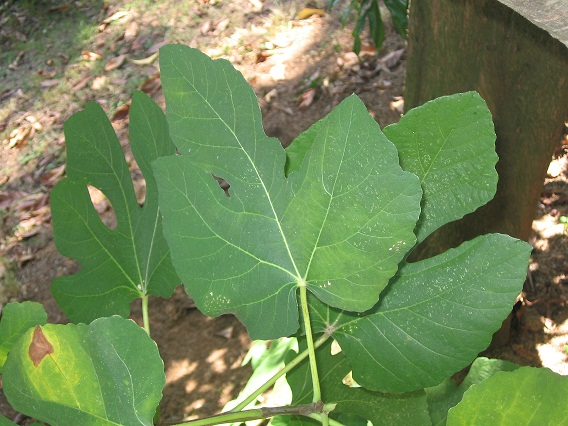
\includegraphics[width=100mm]{leaves.jpg}
	\caption{Caption of the image}
	\label{leave}
\end{center}
\end{figure}

\subsection{Handling bibliography}

Finally, let's find out how a nice bibliography is created. First, check the bibliography styles. A bibliography style tells the document how the references and the list of resources will look like. Currently there exists one style named "alphadin.bst".

In order to set the style do a \textbf{\textbackslash bibliographystyle\{alphadin\}} where "alphadin" (without the ending ".bst") sets the style. If you want to place the bibliography in your text then simply do \textbf{\textbackslash bibliography\{document\}}.

At the time you've created a bibliography (actually, it is created automatically when you create a new project) you can edit its entries by pressing the "Bibliography" button. You can come back here if you press it again. Now that you've entered all your books and articles in the bibliography simply do a \textbf{\textbackslash cite\{refname1\}} where "refname1" specifies the resource you want to cite.

A test: \cite{referenceName1} says that it is a good idea to use LaTeX.

% Create the bibliography right after the text
\bibliographystyle{alphadin}
\bibliography{document}

\end{document}
% All lines that begin with an '%' are comments and won't be displayed in the resulting document1main-branch222

% \documentclass{...} specifies the class of the document. The most common ones are 'book', 'report', 'article' and 'letter'
\documentclass{article}

% Allow the usage of umlauts and other non-ASCII characters
\usepackage[utf8]{inputenc}
% Allow the usage of graphics (.jpg, .png, etc.) in the document
\usepackage{graphicx}
% Allow the change of line spacing
\usepackage{setspace}

% Set line spacing to 1.5xxxneu
\onehalfspacing

% Start the document
\begin{document}

% Show the titlepage (see in 'Documents' below: titlepage.tex)
% Begin a new titlepage. Titlepages have special settings like the absence of page numbers.222
\begin{titlepage}

% Set the text of the page to right-aligned until \end{flushright}
\begin{flushright}

% Set the space between right page border and text to 2.5cm
\rightskip=-2.5cm

% Show an image at this position

\includegraphics[width=50mm]{logo_dark.png}

% Skip a little space
\bigskip
\bigskip
\bigskip
\bigskip

% Create a title for the document and write it in bold font
\LARGE{\textbf{Brief LaTeX Tutorial}}
% Again, do a line break
\linebreak
% Create a subtitle
\large{For LaTeX Beginners}

% Skip some space
\bigskip
\bigskip
\bigskip
\bigskip
\bigskip

% Write in very large letters
\LARGE{verbosus.com}
% Do a line break right after the \LARGE{...} text
\linebreak
% Write in large letters
\large{Free webservices and apps}

% Skip some space
\bigskip
\bigskip
\bigskip
\bigskip
\bigskip
\bigskip

\large{Documentation}

% Skip some space
\bigskip

\normalsize{Vienna, \the\month}

% Skip some space
\bigskip
\bigskip
\bigskip
\bigskip
\bigskip
\bigskip
\bigskip
\bigskip
\bigskip
\bigskip
\bigskip
\bigskip
\bigskip

% Provide some author information
\normalsize{Author:}
\linebreak
\large{Daniel Kuster, MSc}

% End right-alignment at this point
\end{flushright}
% End the title page
\end{titlepage}


% Create a new 1st level heading
\section{First level}

This is the text of the first chapter. If you want to create a subchapter then simply do \textbf{\textbackslash subsection\{Title of first subchapter\}}. If you want to move on to the next chapter then do \textbf{\textbackslash section\{Title of second chapter\}}.

% Create a new 2nd level heading
\subsection{Second level}

Here comes the text of the subsection of the first chapter. Now let's try to insert an image. Currently there exists one image with the name "leaves.jpg" which will be displayed at the current position. This can be changed by changing the [h] (stands for "here", place it at the current position if possible) to a [t] (stands for "top", place it at the beginning of a page if possible), [b] (stands for "bottom", place it at the bottom of a page if possible) or [p] (stands for "float page", place it on a separate page with other floating objects).

The image we've just inserted can be referenced by writing \textbf{\textbackslash ref\{leave\}}. As you can see the figure \ref{leave} shows some leaves.

\subsection{Handling other resource types}

There exist other very useful elements which can be inserted such as tables, itemized lists or description lists. You can try them by simply clicking on the small icons in the editor.

\begin{figure}[htp]
\begin{center}
	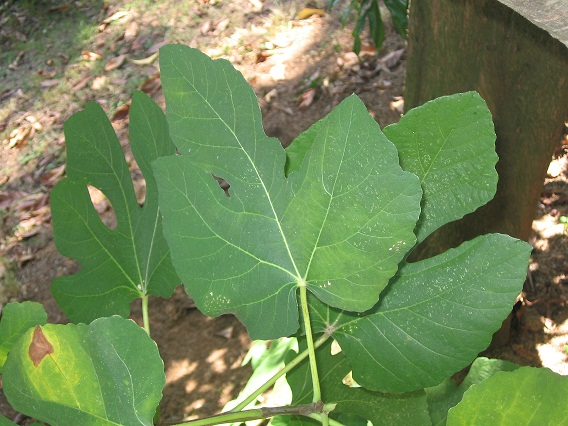
\includegraphics[width=100mm]{leaves.jpg}
	\caption{Caption of the image}
	\label{leave}
\end{center}
\end{figure}

\subsection{Handling bibliography}

Finally, let's find out how a nice bibliography is created. First, check the bibliography styles. A bibliography style tells the document how the references and the list of resources will look like. Currently there exists one style named "alphadin.bst".

In order to set the style do a \textbf{\textbackslash bibliographystyle\{alphadin\}} where "alphadin" (without the ending ".bst") sets the style. If you want to place the bibliography in your text then simply do \textbf{\textbackslash bibliography\{document\}}.

At the time you've created a bibliography (actually, it is created automatically when you create a new project) you can edit its entries by pressing the "Bibliography" button. You can come back here if you press it again. Now that you've entered all your books and articles in the bibliography simply do a \textbf{\textbackslash cite\{refname1\}} where "refname1" specifies the resource you want to cite.

A test: \cite{referenceName1} says that it is a good idea to use LaTeX.

% Create the bibliography right after the text
\bibliographystyle{alphadin}
\bibliography{document}

\end{document}
% All lines that begin with an '%' are comments and won't be displayed in the resulting document1main-branch222

% \documentclass{...} specifies the class of the document. The most common ones are 'book', 'report', 'article' and 'letter'
\documentclass{article}

% Allow the usage of umlauts and other non-ASCII characters
\usepackage[utf8]{inputenc}
% Allow the usage of graphics (.jpg, .png, etc.) in the document
\usepackage{graphicx}
% Allow the change of line spacing
\usepackage{setspace}

% Set line spacing to 1.5xxxneu
\onehalfspacing

% Start the document
\begin{document}

% Show the titlepage (see in 'Documents' below: titlepage.tex)
% Begin a new titlepage. Titlepages have special settings like the absence of page numbers.222
\begin{titlepage}

% Set the text of the page to right-aligned until \end{flushright}
\begin{flushright}

% Set the space between right page border and text to 2.5cm
\rightskip=-2.5cm

% Show an image at this position

\includegraphics[width=50mm]{logo_dark.png}

% Skip a little space
\bigskip
\bigskip
\bigskip
\bigskip

% Create a title for the document and write it in bold font
\LARGE{\textbf{Brief LaTeX Tutorial}}
% Again, do a line break
\linebreak
% Create a subtitle
\large{For LaTeX Beginners}

% Skip some space
\bigskip
\bigskip
\bigskip
\bigskip
\bigskip

% Write in very large letters
\LARGE{verbosus.com}
% Do a line break right after the \LARGE{...} text
\linebreak
% Write in large letters
\large{Free webservices and apps}

% Skip some space
\bigskip
\bigskip
\bigskip
\bigskip
\bigskip
\bigskip

\large{Documentation}

% Skip some space
\bigskip

\normalsize{Vienna, \the\month}

% Skip some space
\bigskip
\bigskip
\bigskip
\bigskip
\bigskip
\bigskip
\bigskip
\bigskip
\bigskip
\bigskip
\bigskip
\bigskip
\bigskip

% Provide some author information
\normalsize{Author:}
\linebreak
\large{Daniel Kuster, MSc}

% End right-alignment at this point
\end{flushright}
% End the title page
\end{titlepage}


% Create a new 1st level heading
\section{First level}

This is the text of the first chapter. If you want to create a subchapter then simply do \textbf{\textbackslash subsection\{Title of first subchapter\}}. If you want to move on to the next chapter then do \textbf{\textbackslash section\{Title of second chapter\}}.

% Create a new 2nd level heading
\subsection{Second level}

Here comes the text of the subsection of the first chapter. Now let's try to insert an image. Currently there exists one image with the name "leaves.jpg" which will be displayed at the current position. This can be changed by changing the [h] (stands for "here", place it at the current position if possible) to a [t] (stands for "top", place it at the beginning of a page if possible), [b] (stands for "bottom", place it at the bottom of a page if possible) or [p] (stands for "float page", place it on a separate page with other floating objects).

The image we've just inserted can be referenced by writing \textbf{\textbackslash ref\{leave\}}. As you can see the figure \ref{leave} shows some leaves.

\subsection{Handling other resource types}

There exist other very useful elements which can be inserted such as tables, itemized lists or description lists. You can try them by simply clicking on the small icons in the editor.

\begin{figure}[htp]
\begin{center}
	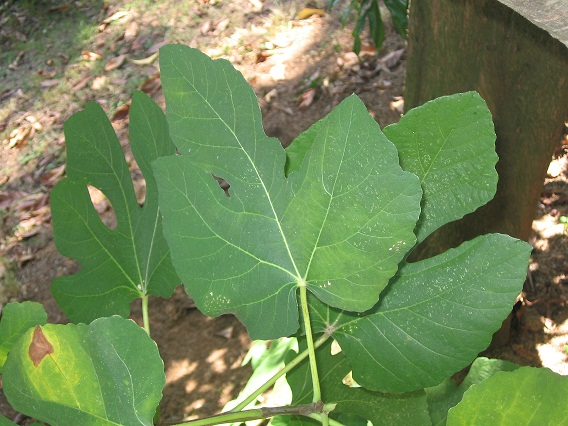
\includegraphics[width=100mm]{leaves.jpg}
	\caption{Caption of the image}
	\label{leave}
\end{center}
\end{figure}

\subsection{Handling bibliography}

Finally, let's find out how a nice bibliography is created. First, check the bibliography styles. A bibliography style tells the document how the references and the list of resources will look like. Currently there exists one style named "alphadin.bst".

In order to set the style do a \textbf{\textbackslash bibliographystyle\{alphadin\}} where "alphadin" (without the ending ".bst") sets the style. If you want to place the bibliography in your text then simply do \textbf{\textbackslash bibliography\{document\}}.

At the time you've created a bibliography (actually, it is created automatically when you create a new project) you can edit its entries by pressing the "Bibliography" button. You can come back here if you press it again. Now that you've entered all your books and articles in the bibliography simply do a \textbf{\textbackslash cite\{refname1\}} where "refname1" specifies the resource you want to cite.

A test: \cite{referenceName1} says that it is a good idea to use LaTeX.

% Create the bibliography right after the text
\bibliographystyle{alphadin}
\bibliography{document}

\end{document}
% All lines that begin with an '%' are comments and won't be displayed in the resulting document1main-branch222

% \documentclass{...} specifies the class of the document. The most common ones are 'book', 'report', 'article' and 'letter'
\documentclass{article}

% Allow the usage of umlauts and other non-ASCII characters
\usepackage[utf8]{inputenc}
% Allow the usage of graphics (.jpg, .png, etc.) in the document
\usepackage{graphicx}
% Allow the change of line spacing
\usepackage{setspace}

% Set line spacing to 1.5xxxneu
\onehalfspacing

% Start the document
\begin{document}

% Show the titlepage (see in 'Documents' below: titlepage.tex)
% Begin a new titlepage. Titlepages have special settings like the absence of page numbers.222
\begin{titlepage}

% Set the text of the page to right-aligned until \end{flushright}
\begin{flushright}

% Set the space between right page border and text to 2.5cm
\rightskip=-2.5cm

% Show an image at this position

\includegraphics[width=50mm]{logo_dark.png}

% Skip a little space
\bigskip
\bigskip
\bigskip
\bigskip

% Create a title for the document and write it in bold font
\LARGE{\textbf{Brief LaTeX Tutorial}}
% Again, do a line break
\linebreak
% Create a subtitle
\large{For LaTeX Beginners}

% Skip some space
\bigskip
\bigskip
\bigskip
\bigskip
\bigskip

% Write in very large letters
\LARGE{verbosus.com}
% Do a line break right after the \LARGE{...} text
\linebreak
% Write in large letters
\large{Free webservices and apps}

% Skip some space
\bigskip
\bigskip
\bigskip
\bigskip
\bigskip
\bigskip

\large{Documentation}

% Skip some space
\bigskip

\normalsize{Vienna, \the\month}

% Skip some space
\bigskip
\bigskip
\bigskip
\bigskip
\bigskip
\bigskip
\bigskip
\bigskip
\bigskip
\bigskip
\bigskip
\bigskip
\bigskip

% Provide some author information
\normalsize{Author:}
\linebreak
\large{Daniel Kuster, MSc}

% End right-alignment at this point
\end{flushright}
% End the title page
\end{titlepage}


% Create a new 1st level heading
\section{First level}

This is the text of the first chapter. If you want to create a subchapter then simply do \textbf{\textbackslash subsection\{Title of first subchapter\}}. If you want to move on to the next chapter then do \textbf{\textbackslash section\{Title of second chapter\}}.

% Create a new 2nd level heading
\subsection{Second level}

Here comes the text of the subsection of the first chapter. Now let's try to insert an image. Currently there exists one image with the name "leaves.jpg" which will be displayed at the current position. This can be changed by changing the [h] (stands for "here", place it at the current position if possible) to a [t] (stands for "top", place it at the beginning of a page if possible), [b] (stands for "bottom", place it at the bottom of a page if possible) or [p] (stands for "float page", place it on a separate page with other floating objects).

The image we've just inserted can be referenced by writing \textbf{\textbackslash ref\{leave\}}. As you can see the figure \ref{leave} shows some leaves.

\subsection{Handling other resource types}

There exist other very useful elements which can be inserted such as tables, itemized lists or description lists. You can try them by simply clicking on the small icons in the editor.

\begin{figure}[htp]
\begin{center}
	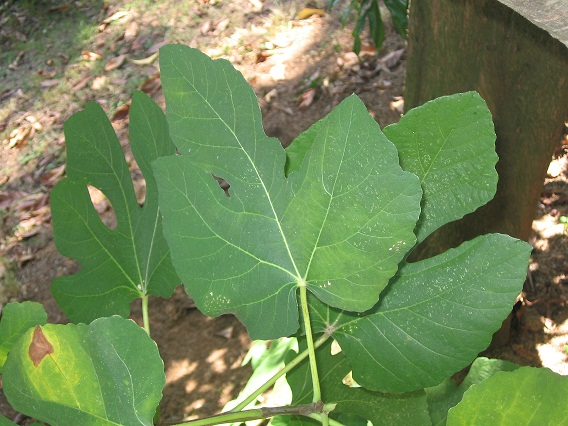
\includegraphics[width=100mm]{leaves.jpg}
	\caption{Caption of the image}
	\label{leave}
\end{center}
\end{figure}

\subsection{Handling bibliography}

Finally, let's find out how a nice bibliography is created. First, check the bibliography styles. A bibliography style tells the document how the references and the list of resources will look like. Currently there exists one style named "alphadin.bst".

In order to set the style do a \textbf{\textbackslash bibliographystyle\{alphadin\}} where "alphadin" (without the ending ".bst") sets the style. If you want to place the bibliography in your text then simply do \textbf{\textbackslash bibliography\{document\}}.

At the time you've created a bibliography (actually, it is created automatically when you create a new project) you can edit its entries by pressing the "Bibliography" button. You can come back here if you press it again. Now that you've entered all your books and articles in the bibliography simply do a \textbf{\textbackslash cite\{refname1\}} where "refname1" specifies the resource you want to cite.

A test: \cite{referenceName1} says that it is a good idea to use LaTeX.

% Create the bibliography right after the text
\bibliographystyle{alphadin}
\bibliography{document}

\end{document}
% All lines that begin with an '%' are comments and won't be displayed in the resulting document1main-branch222

% \documentclass{...} specifies the class of the document. The most common ones are 'book', 'report', 'article' and 'letter'
\documentclass{article}

% Allow the usage of umlauts and other non-ASCII characters
\usepackage[utf8]{inputenc}
% Allow the usage of graphics (.jpg, .png, etc.) in the document
\usepackage{graphicx}
% Allow the change of line spacing
\usepackage{setspace}

% Set line spacing to 1.5xxxneu
\onehalfspacing

% Start the document
\begin{document}

% Show the titlepage (see in 'Documents' below: titlepage.tex)
% Begin a new titlepage. Titlepages have special settings like the absence of page numbers.222
\begin{titlepage}

% Set the text of the page to right-aligned until \end{flushright}
\begin{flushright}

% Set the space between right page border and text to 2.5cm
\rightskip=-2.5cm

% Show an image at this position

\includegraphics[width=50mm]{logo_dark.png}

% Skip a little space
\bigskip
\bigskip
\bigskip
\bigskip

% Create a title for the document and write it in bold font
\LARGE{\textbf{Brief LaTeX Tutorial}}
% Again, do a line break
\linebreak
% Create a subtitle
\large{For LaTeX Beginners}

% Skip some space
\bigskip
\bigskip
\bigskip
\bigskip
\bigskip

% Write in very large letters
\LARGE{verbosus.com}
% Do a line break right after the \LARGE{...} text
\linebreak
% Write in large letters
\large{Free webservices and apps}

% Skip some space
\bigskip
\bigskip
\bigskip
\bigskip
\bigskip
\bigskip

\large{Documentation}

% Skip some space
\bigskip

\normalsize{Vienna, \the\month}

% Skip some space
\bigskip
\bigskip
\bigskip
\bigskip
\bigskip
\bigskip
\bigskip
\bigskip
\bigskip
\bigskip
\bigskip
\bigskip
\bigskip

% Provide some author information
\normalsize{Author:}
\linebreak
\large{Daniel Kuster, MSc}

% End right-alignment at this point
\end{flushright}
% End the title page
\end{titlepage}


% Create a new 1st level heading
\section{First level}

This is the text of the first chapter. If you want to create a subchapter then simply do \textbf{\textbackslash subsection\{Title of first subchapter\}}. If you want to move on to the next chapter then do \textbf{\textbackslash section\{Title of second chapter\}}.

% Create a new 2nd level heading
\subsection{Second level}

Here comes the text of the subsection of the first chapter. Now let's try to insert an image. Currently there exists one image with the name "leaves.jpg" which will be displayed at the current position. This can be changed by changing the [h] (stands for "here", place it at the current position if possible) to a [t] (stands for "top", place it at the beginning of a page if possible), [b] (stands for "bottom", place it at the bottom of a page if possible) or [p] (stands for "float page", place it on a separate page with other floating objects).

The image we've just inserted can be referenced by writing \textbf{\textbackslash ref\{leave\}}. As you can see the figure \ref{leave} shows some leaves.

\subsection{Handling other resource types}

There exist other very useful elements which can be inserted such as tables, itemized lists or description lists. You can try them by simply clicking on the small icons in the editor.

\begin{figure}[htp]
\begin{center}
	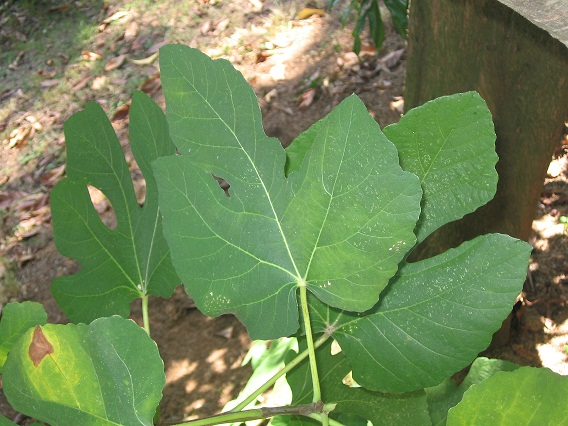
\includegraphics[width=100mm]{leaves.jpg}
	\caption{Caption of the image}
	\label{leave}
\end{center}
\end{figure}

\subsection{Handling bibliography}

Finally, let's find out how a nice bibliography is created. First, check the bibliography styles. A bibliography style tells the document how the references and the list of resources will look like. Currently there exists one style named "alphadin.bst".

In order to set the style do a \textbf{\textbackslash bibliographystyle\{alphadin\}} where "alphadin" (without the ending ".bst") sets the style. If you want to place the bibliography in your text then simply do \textbf{\textbackslash bibliography\{document\}}.

At the time you've created a bibliography (actually, it is created automatically when you create a new project) you can edit its entries by pressing the "Bibliography" button. You can come back here if you press it again. Now that you've entered all your books and articles in the bibliography simply do a \textbf{\textbackslash cite\{refname1\}} where "refname1" specifies the resource you want to cite.

A test: \cite{referenceName1} says that it is a good idea to use LaTeX.

% Create the bibliography right after the text
\bibliographystyle{alphadin}
\bibliography{document}

\end{document}
% All lines that begin with an '%' are comments and won't be displayed in the resulting document1main-branch222

% \documentclass{...} specifies the class of the document. The most common ones are 'book', 'report', 'article' and 'letter'
\documentclass{article}

% Allow the usage of umlauts and other non-ASCII characters
\usepackage[utf8]{inputenc}
% Allow the usage of graphics (.jpg, .png, etc.) in the document
\usepackage{graphicx}
% Allow the change of line spacing
\usepackage{setspace}

% Set line spacing to 1.5xxxneu
\onehalfspacing

% Start the document
\begin{document}

% Show the titlepage (see in 'Documents' below: titlepage.tex)
% Begin a new titlepage. Titlepages have special settings like the absence of page numbers.222
\begin{titlepage}

% Set the text of the page to right-aligned until \end{flushright}
\begin{flushright}

% Set the space between right page border and text to 2.5cm
\rightskip=-2.5cm

% Show an image at this position

\includegraphics[width=50mm]{logo_dark.png}

% Skip a little space
\bigskip
\bigskip
\bigskip
\bigskip

% Create a title for the document and write it in bold font
\LARGE{\textbf{Brief LaTeX Tutorial}}
% Again, do a line break
\linebreak
% Create a subtitle
\large{For LaTeX Beginners}

% Skip some space
\bigskip
\bigskip
\bigskip
\bigskip
\bigskip

% Write in very large letters
\LARGE{verbosus.com}
% Do a line break right after the \LARGE{...} text
\linebreak
% Write in large letters
\large{Free webservices and apps}

% Skip some space
\bigskip
\bigskip
\bigskip
\bigskip
\bigskip
\bigskip

\large{Documentation}

% Skip some space
\bigskip

\normalsize{Vienna, \the\month}

% Skip some space
\bigskip
\bigskip
\bigskip
\bigskip
\bigskip
\bigskip
\bigskip
\bigskip
\bigskip
\bigskip
\bigskip
\bigskip
\bigskip

% Provide some author information
\normalsize{Author:}
\linebreak
\large{Daniel Kuster, MSc}

% End right-alignment at this point
\end{flushright}
% End the title page
\end{titlepage}


% Create a new 1st level heading
\section{First level}

This is the text of the first chapter. If you want to create a subchapter then simply do \textbf{\textbackslash subsection\{Title of first subchapter\}}. If you want to move on to the next chapter then do \textbf{\textbackslash section\{Title of second chapter\}}.

% Create a new 2nd level heading
\subsection{Second level}

Here comes the text of the subsection of the first chapter. Now let's try to insert an image. Currently there exists one image with the name "leaves.jpg" which will be displayed at the current position. This can be changed by changing the [h] (stands for "here", place it at the current position if possible) to a [t] (stands for "top", place it at the beginning of a page if possible), [b] (stands for "bottom", place it at the bottom of a page if possible) or [p] (stands for "float page", place it on a separate page with other floating objects).

The image we've just inserted can be referenced by writing \textbf{\textbackslash ref\{leave\}}. As you can see the figure \ref{leave} shows some leaves.

\subsection{Handling other resource types}

There exist other very useful elements which can be inserted such as tables, itemized lists or description lists. You can try them by simply clicking on the small icons in the editor.

\begin{figure}[htp]
\begin{center}
	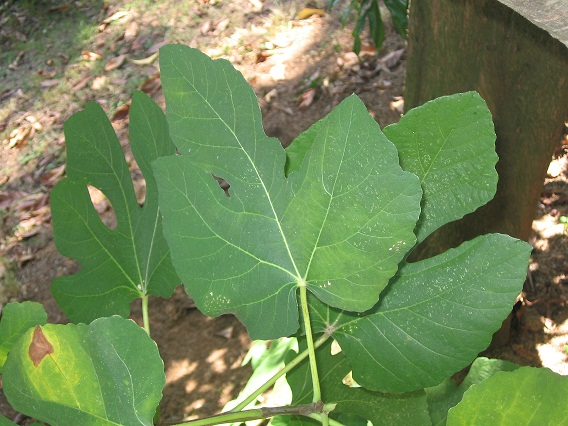
\includegraphics[width=100mm]{leaves.jpg}
	\caption{Caption of the image}
	\label{leave}
\end{center}
\end{figure}

\subsection{Handling bibliography}

Finally, let's find out how a nice bibliography is created. First, check the bibliography styles. A bibliography style tells the document how the references and the list of resources will look like. Currently there exists one style named "alphadin.bst".

In order to set the style do a \textbf{\textbackslash bibliographystyle\{alphadin\}} where "alphadin" (without the ending ".bst") sets the style. If you want to place the bibliography in your text then simply do \textbf{\textbackslash bibliography\{document\}}.

At the time you've created a bibliography (actually, it is created automatically when you create a new project) you can edit its entries by pressing the "Bibliography" button. You can come back here if you press it again. Now that you've entered all your books and articles in the bibliography simply do a \textbf{\textbackslash cite\{refname1\}} where "refname1" specifies the resource you want to cite.

A test: \cite{referenceName1} says that it is a good idea to use LaTeX.

% Create the bibliography right after the text
\bibliographystyle{alphadin}
\bibliography{document}

\end{document}
% All lines that begin with an '%' are comments and won't be displayed in the resulting document1main-branch222

% \documentclass{...} specifies the class of the document. The most common ones are 'book', 'report', 'article' and 'letter'
\documentclass{article}

% Allow the usage of umlauts and other non-ASCII characters
\usepackage[utf8]{inputenc}
% Allow the usage of graphics (.jpg, .png, etc.) in the document
\usepackage{graphicx}
% Allow the change of line spacing
\usepackage{setspace}

% Set line spacing to 1.5xxxneu
\onehalfspacing

% Start the document
\begin{document}

% Show the titlepage (see in 'Documents' below: titlepage.tex)
% Begin a new titlepage. Titlepages have special settings like the absence of page numbers.222
\begin{titlepage}

% Set the text of the page to right-aligned until \end{flushright}
\begin{flushright}

% Set the space between right page border and text to 2.5cm
\rightskip=-2.5cm

% Show an image at this position

\includegraphics[width=50mm]{logo_dark.png}

% Skip a little space
\bigskip
\bigskip
\bigskip
\bigskip

% Create a title for the document and write it in bold font
\LARGE{\textbf{Brief LaTeX Tutorial}}
% Again, do a line break
\linebreak
% Create a subtitle
\large{For LaTeX Beginners}

% Skip some space
\bigskip
\bigskip
\bigskip
\bigskip
\bigskip

% Write in very large letters
\LARGE{verbosus.com}
% Do a line break right after the \LARGE{...} text
\linebreak
% Write in large letters
\large{Free webservices and apps}

% Skip some space
\bigskip
\bigskip
\bigskip
\bigskip
\bigskip
\bigskip

\large{Documentation}

% Skip some space
\bigskip

\normalsize{Vienna, \the\month}

% Skip some space
\bigskip
\bigskip
\bigskip
\bigskip
\bigskip
\bigskip
\bigskip
\bigskip
\bigskip
\bigskip
\bigskip
\bigskip
\bigskip

% Provide some author information
\normalsize{Author:}
\linebreak
\large{Daniel Kuster, MSc}

% End right-alignment at this point
\end{flushright}
% End the title page
\end{titlepage}


% Create a new 1st level heading
\section{First level}

This is the text of the first chapter. If you want to create a subchapter then simply do \textbf{\textbackslash subsection\{Title of first subchapter\}}. If you want to move on to the next chapter then do \textbf{\textbackslash section\{Title of second chapter\}}.

% Create a new 2nd level heading
\subsection{Second level}

Here comes the text of the subsection of the first chapter. Now let's try to insert an image. Currently there exists one image with the name "leaves.jpg" which will be displayed at the current position. This can be changed by changing the [h] (stands for "here", place it at the current position if possible) to a [t] (stands for "top", place it at the beginning of a page if possible), [b] (stands for "bottom", place it at the bottom of a page if possible) or [p] (stands for "float page", place it on a separate page with other floating objects).

The image we've just inserted can be referenced by writing \textbf{\textbackslash ref\{leave\}}. As you can see the figure \ref{leave} shows some leaves.

\subsection{Handling other resource types}

There exist other very useful elements which can be inserted such as tables, itemized lists or description lists. You can try them by simply clicking on the small icons in the editor.

\begin{figure}[htp]
\begin{center}
	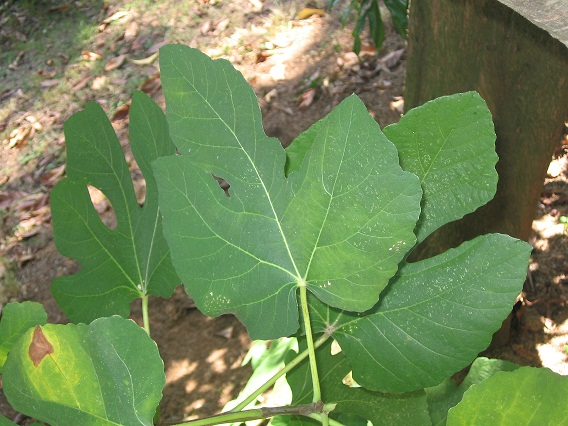
\includegraphics[width=100mm]{leaves.jpg}
	\caption{Caption of the image}
	\label{leave}
\end{center}
\end{figure}

\subsection{Handling bibliography}

Finally, let's find out how a nice bibliography is created. First, check the bibliography styles. A bibliography style tells the document how the references and the list of resources will look like. Currently there exists one style named "alphadin.bst".

In order to set the style do a \textbf{\textbackslash bibliographystyle\{alphadin\}} where "alphadin" (without the ending ".bst") sets the style. If you want to place the bibliography in your text then simply do \textbf{\textbackslash bibliography\{document\}}.

At the time you've created a bibliography (actually, it is created automatically when you create a new project) you can edit its entries by pressing the "Bibliography" button. You can come back here if you press it again. Now that you've entered all your books and articles in the bibliography simply do a \textbf{\textbackslash cite\{refname1\}} where "refname1" specifies the resource you want to cite.

A test: \cite{referenceName1} says that it is a good idea to use LaTeX.

% Create the bibliography right after the text
\bibliographystyle{alphadin}
\bibliography{document}

\end{document}
% All lines that begin with an '%' are comments and won't be displayed in the resulting document1main-branch222

% \documentclass{...} specifies the class of the document. The most common ones are 'book', 'report', 'article' and 'letter'
\documentclass{article}

% Allow the usage of umlauts and other non-ASCII characters
\usepackage[utf8]{inputenc}
% Allow the usage of graphics (.jpg, .png, etc.) in the document
\usepackage{graphicx}
% Allow the change of line spacing
\usepackage{setspace}

% Set line spacing to 1.5xxxneu
\onehalfspacing

% Start the document
\begin{document}

% Show the titlepage (see in 'Documents' below: titlepage.tex)
% Begin a new titlepage. Titlepages have special settings like the absence of page numbers.222
\begin{titlepage}

% Set the text of the page to right-aligned until \end{flushright}
\begin{flushright}

% Set the space between right page border and text to 2.5cm
\rightskip=-2.5cm

% Show an image at this position

\includegraphics[width=50mm]{logo_dark.png}

% Skip a little space
\bigskip
\bigskip
\bigskip
\bigskip

% Create a title for the document and write it in bold font
\LARGE{\textbf{Brief LaTeX Tutorial}}
% Again, do a line break
\linebreak
% Create a subtitle
\large{For LaTeX Beginners}

% Skip some space
\bigskip
\bigskip
\bigskip
\bigskip
\bigskip

% Write in very large letters
\LARGE{verbosus.com}
% Do a line break right after the \LARGE{...} text
\linebreak
% Write in large letters
\large{Free webservices and apps}

% Skip some space
\bigskip
\bigskip
\bigskip
\bigskip
\bigskip
\bigskip

\large{Documentation}

% Skip some space
\bigskip

\normalsize{Vienna, \the\month}

% Skip some space
\bigskip
\bigskip
\bigskip
\bigskip
\bigskip
\bigskip
\bigskip
\bigskip
\bigskip
\bigskip
\bigskip
\bigskip
\bigskip

% Provide some author information
\normalsize{Author:}
\linebreak
\large{Daniel Kuster, MSc}

% End right-alignment at this point
\end{flushright}
% End the title page
\end{titlepage}


% Create a new 1st level heading
\section{First level}

This is the text of the first chapter. If you want to create a subchapter then simply do \textbf{\textbackslash subsection\{Title of first subchapter\}}. If you want to move on to the next chapter then do \textbf{\textbackslash section\{Title of second chapter\}}.

% Create a new 2nd level heading
\subsection{Second level}

Here comes the text of the subsection of the first chapter. Now let's try to insert an image. Currently there exists one image with the name "leaves.jpg" which will be displayed at the current position. This can be changed by changing the [h] (stands for "here", place it at the current position if possible) to a [t] (stands for "top", place it at the beginning of a page if possible), [b] (stands for "bottom", place it at the bottom of a page if possible) or [p] (stands for "float page", place it on a separate page with other floating objects).

The image we've just inserted can be referenced by writing \textbf{\textbackslash ref\{leave\}}. As you can see the figure \ref{leave} shows some leaves.

\subsection{Handling other resource types}

There exist other very useful elements which can be inserted such as tables, itemized lists or description lists. You can try them by simply clicking on the small icons in the editor.

\begin{figure}[htp]
\begin{center}
	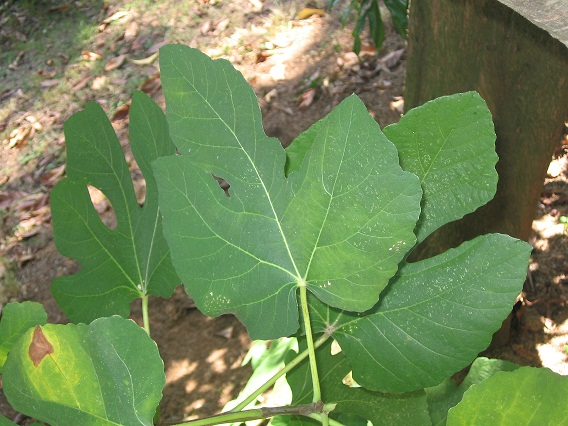
\includegraphics[width=100mm]{leaves.jpg}
	\caption{Caption of the image}
	\label{leave}
\end{center}
\end{figure}

\subsection{Handling bibliography}

Finally, let's find out how a nice bibliography is created. First, check the bibliography styles. A bibliography style tells the document how the references and the list of resources will look like. Currently there exists one style named "alphadin.bst".

In order to set the style do a \textbf{\textbackslash bibliographystyle\{alphadin\}} where "alphadin" (without the ending ".bst") sets the style. If you want to place the bibliography in your text then simply do \textbf{\textbackslash bibliography\{document\}}.

At the time you've created a bibliography (actually, it is created automatically when you create a new project) you can edit its entries by pressing the "Bibliography" button. You can come back here if you press it again. Now that you've entered all your books and articles in the bibliography simply do a \textbf{\textbackslash cite\{refname1\}} where "refname1" specifies the resource you want to cite.

A test: \cite{referenceName1} says that it is a good idea to use LaTeX.

% Create the bibliography right after the text
\bibliographystyle{alphadin}
\bibliography{document}

\end{document}
% All lines that begin with an '%' are comments and won't be displayed in the resulting document1main-branch222

% \documentclass{...} specifies the class of the document. The most common ones are 'book', 'report', 'article' and 'letter'
\documentclass{article}

% Allow the usage of umlauts and other non-ASCII characters
\usepackage[utf8]{inputenc}
% Allow the usage of graphics (.jpg, .png, etc.) in the document
\usepackage{graphicx}
% Allow the change of line spacing
\usepackage{setspace}

% Set line spacing to 1.5xxxneu
\onehalfspacing

% Start the document
\begin{document}

% Show the titlepage (see in 'Documents' below: titlepage.tex)
% Begin a new titlepage. Titlepages have special settings like the absence of page numbers.222
\begin{titlepage}

% Set the text of the page to right-aligned until \end{flushright}
\begin{flushright}

% Set the space between right page border and text to 2.5cm
\rightskip=-2.5cm

% Show an image at this position

\includegraphics[width=50mm]{logo_dark.png}

% Skip a little space
\bigskip
\bigskip
\bigskip
\bigskip

% Create a title for the document and write it in bold font
\LARGE{\textbf{Brief LaTeX Tutorial}}
% Again, do a line break
\linebreak
% Create a subtitle
\large{For LaTeX Beginners}

% Skip some space
\bigskip
\bigskip
\bigskip
\bigskip
\bigskip

% Write in very large letters
\LARGE{verbosus.com}
% Do a line break right after the \LARGE{...} text
\linebreak
% Write in large letters
\large{Free webservices and apps}

% Skip some space
\bigskip
\bigskip
\bigskip
\bigskip
\bigskip
\bigskip

\large{Documentation}

% Skip some space
\bigskip

\normalsize{Vienna, \the\month}

% Skip some space
\bigskip
\bigskip
\bigskip
\bigskip
\bigskip
\bigskip
\bigskip
\bigskip
\bigskip
\bigskip
\bigskip
\bigskip
\bigskip

% Provide some author information
\normalsize{Author:}
\linebreak
\large{Daniel Kuster, MSc}

% End right-alignment at this point
\end{flushright}
% End the title page
\end{titlepage}


% Create a new 1st level heading
\section{First level}

This is the text of the first chapter. If you want to create a subchapter then simply do \textbf{\textbackslash subsection\{Title of first subchapter\}}. If you want to move on to the next chapter then do \textbf{\textbackslash section\{Title of second chapter\}}.

% Create a new 2nd level heading
\subsection{Second level}

Here comes the text of the subsection of the first chapter. Now let's try to insert an image. Currently there exists one image with the name "leaves.jpg" which will be displayed at the current position. This can be changed by changing the [h] (stands for "here", place it at the current position if possible) to a [t] (stands for "top", place it at the beginning of a page if possible), [b] (stands for "bottom", place it at the bottom of a page if possible) or [p] (stands for "float page", place it on a separate page with other floating objects).

The image we've just inserted can be referenced by writing \textbf{\textbackslash ref\{leave\}}. As you can see the figure \ref{leave} shows some leaves.

\subsection{Handling other resource types}

There exist other very useful elements which can be inserted such as tables, itemized lists or description lists. You can try them by simply clicking on the small icons in the editor.

\begin{figure}[htp]
\begin{center}
	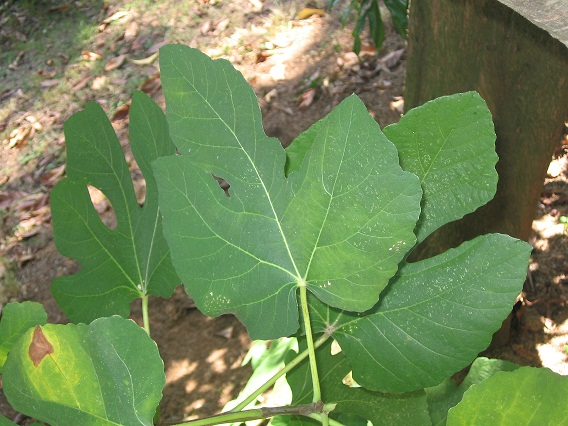
\includegraphics[width=100mm]{leaves.jpg}
	\caption{Caption of the image}
	\label{leave}
\end{center}
\end{figure}

\subsection{Handling bibliography}

Finally, let's find out how a nice bibliography is created. First, check the bibliography styles. A bibliography style tells the document how the references and the list of resources will look like. Currently there exists one style named "alphadin.bst".

In order to set the style do a \textbf{\textbackslash bibliographystyle\{alphadin\}} where "alphadin" (without the ending ".bst") sets the style. If you want to place the bibliography in your text then simply do \textbf{\textbackslash bibliography\{document\}}.

At the time you've created a bibliography (actually, it is created automatically when you create a new project) you can edit its entries by pressing the "Bibliography" button. You can come back here if you press it again. Now that you've entered all your books and articles in the bibliography simply do a \textbf{\textbackslash cite\{refname1\}} where "refname1" specifies the resource you want to cite.

A test: \cite{referenceName1} says that it is a good idea to use LaTeX.

% Create the bibliography right after the text
\bibliographystyle{alphadin}
\bibliography{document}

\end{document}
% All lines that begin with an '%' are comments and won't be displayed in the resulting document1main-branch222

% \documentclass{...} specifies the class of the document. The most common ones are 'book', 'report', 'article' and 'letter'
\documentclass{article}

% Allow the usage of umlauts and other non-ASCII characters
\usepackage[utf8]{inputenc}
% Allow the usage of graphics (.jpg, .png, etc.) in the document
\usepackage{graphicx}
% Allow the change of line spacing
\usepackage{setspace}

% Set line spacing to 1.5xxxneu
\onehalfspacing

% Start the document
\begin{document}

% Show the titlepage (see in 'Documents' below: titlepage.tex)
% Begin a new titlepage. Titlepages have special settings like the absence of page numbers.222
\begin{titlepage}

% Set the text of the page to right-aligned until \end{flushright}
\begin{flushright}

% Set the space between right page border and text to 2.5cm
\rightskip=-2.5cm

% Show an image at this position

\includegraphics[width=50mm]{logo_dark.png}

% Skip a little space
\bigskip
\bigskip
\bigskip
\bigskip

% Create a title for the document and write it in bold font
\LARGE{\textbf{Brief LaTeX Tutorial}}
% Again, do a line break
\linebreak
% Create a subtitle
\large{For LaTeX Beginners}

% Skip some space
\bigskip
\bigskip
\bigskip
\bigskip
\bigskip

% Write in very large letters
\LARGE{verbosus.com}
% Do a line break right after the \LARGE{...} text
\linebreak
% Write in large letters
\large{Free webservices and apps}

% Skip some space
\bigskip
\bigskip
\bigskip
\bigskip
\bigskip
\bigskip

\large{Documentation}

% Skip some space
\bigskip

\normalsize{Vienna, \the\month}

% Skip some space
\bigskip
\bigskip
\bigskip
\bigskip
\bigskip
\bigskip
\bigskip
\bigskip
\bigskip
\bigskip
\bigskip
\bigskip
\bigskip

% Provide some author information
\normalsize{Author:}
\linebreak
\large{Daniel Kuster, MSc}

% End right-alignment at this point
\end{flushright}
% End the title page
\end{titlepage}


% Create a new 1st level heading
\section{First level}

This is the text of the first chapter. If you want to create a subchapter then simply do \textbf{\textbackslash subsection\{Title of first subchapter\}}. If you want to move on to the next chapter then do \textbf{\textbackslash section\{Title of second chapter\}}.

% Create a new 2nd level heading
\subsection{Second level}

Here comes the text of the subsection of the first chapter. Now let's try to insert an image. Currently there exists one image with the name "leaves.jpg" which will be displayed at the current position. This can be changed by changing the [h] (stands for "here", place it at the current position if possible) to a [t] (stands for "top", place it at the beginning of a page if possible), [b] (stands for "bottom", place it at the bottom of a page if possible) or [p] (stands for "float page", place it on a separate page with other floating objects).

The image we've just inserted can be referenced by writing \textbf{\textbackslash ref\{leave\}}. As you can see the figure \ref{leave} shows some leaves.

\subsection{Handling other resource types}

There exist other very useful elements which can be inserted such as tables, itemized lists or description lists. You can try them by simply clicking on the small icons in the editor.

\begin{figure}[htp]
\begin{center}
	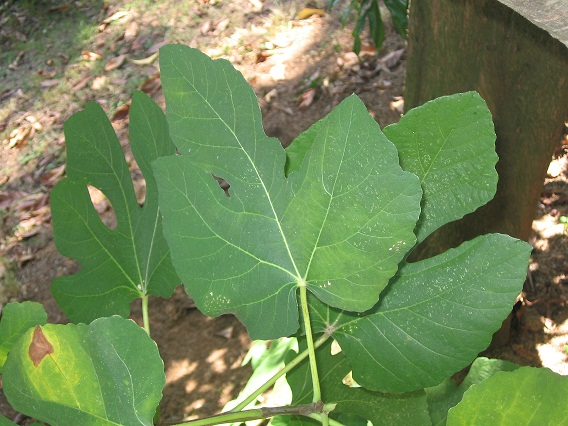
\includegraphics[width=100mm]{leaves.jpg}
	\caption{Caption of the image}
	\label{leave}
\end{center}
\end{figure}

\subsection{Handling bibliography}

Finally, let's find out how a nice bibliography is created. First, check the bibliography styles. A bibliography style tells the document how the references and the list of resources will look like. Currently there exists one style named "alphadin.bst".

In order to set the style do a \textbf{\textbackslash bibliographystyle\{alphadin\}} where "alphadin" (without the ending ".bst") sets the style. If you want to place the bibliography in your text then simply do \textbf{\textbackslash bibliography\{document\}}.

At the time you've created a bibliography (actually, it is created automatically when you create a new project) you can edit its entries by pressing the "Bibliography" button. You can come back here if you press it again. Now that you've entered all your books and articles in the bibliography simply do a \textbf{\textbackslash cite\{refname1\}} where "refname1" specifies the resource you want to cite.

A test: \cite{referenceName1} says that it is a good idea to use LaTeX.

% Create the bibliography right after the text
\bibliographystyle{alphadin}
\bibliography{document}

\end{document}
% All lines that begin with an '%' are comments and won't be displayed in the resulting document1main-branch222

% \documentclass{...} specifies the class of the document. The most common ones are 'book', 'report', 'article' and 'letter'
\documentclass{article}

% Allow the usage of umlauts and other non-ASCII characters
\usepackage[utf8]{inputenc}
% Allow the usage of graphics (.jpg, .png, etc.) in the document
\usepackage{graphicx}
% Allow the change of line spacing
\usepackage{setspace}

% Set line spacing to 1.5xxxneu
\onehalfspacing

% Start the document
\begin{document}

% Show the titlepage (see in 'Documents' below: titlepage.tex)
% Begin a new titlepage. Titlepages have special settings like the absence of page numbers.222
\begin{titlepage}

% Set the text of the page to right-aligned until \end{flushright}
\begin{flushright}

% Set the space between right page border and text to 2.5cm
\rightskip=-2.5cm

% Show an image at this position

\includegraphics[width=50mm]{logo_dark.png}

% Skip a little space
\bigskip
\bigskip
\bigskip
\bigskip

% Create a title for the document and write it in bold font
\LARGE{\textbf{Brief LaTeX Tutorial}}
% Again, do a line break
\linebreak
% Create a subtitle
\large{For LaTeX Beginners}

% Skip some space
\bigskip
\bigskip
\bigskip
\bigskip
\bigskip

% Write in very large letters
\LARGE{verbosus.com}
% Do a line break right after the \LARGE{...} text
\linebreak
% Write in large letters
\large{Free webservices and apps}

% Skip some space
\bigskip
\bigskip
\bigskip
\bigskip
\bigskip
\bigskip

\large{Documentation}

% Skip some space
\bigskip

\normalsize{Vienna, \the\month}

% Skip some space
\bigskip
\bigskip
\bigskip
\bigskip
\bigskip
\bigskip
\bigskip
\bigskip
\bigskip
\bigskip
\bigskip
\bigskip
\bigskip

% Provide some author information
\normalsize{Author:}
\linebreak
\large{Daniel Kuster, MSc}

% End right-alignment at this point
\end{flushright}
% End the title page
\end{titlepage}


% Create a new 1st level heading
\section{First level}

This is the text of the first chapter. If you want to create a subchapter then simply do \textbf{\textbackslash subsection\{Title of first subchapter\}}. If you want to move on to the next chapter then do \textbf{\textbackslash section\{Title of second chapter\}}.

% Create a new 2nd level heading
\subsection{Second level}

Here comes the text of the subsection of the first chapter. Now let's try to insert an image. Currently there exists one image with the name "leaves.jpg" which will be displayed at the current position. This can be changed by changing the [h] (stands for "here", place it at the current position if possible) to a [t] (stands for "top", place it at the beginning of a page if possible), [b] (stands for "bottom", place it at the bottom of a page if possible) or [p] (stands for "float page", place it on a separate page with other floating objects).

The image we've just inserted can be referenced by writing \textbf{\textbackslash ref\{leave\}}. As you can see the figure \ref{leave} shows some leaves.

\subsection{Handling other resource types}

There exist other very useful elements which can be inserted such as tables, itemized lists or description lists. You can try them by simply clicking on the small icons in the editor.

\begin{figure}[htp]
\begin{center}
	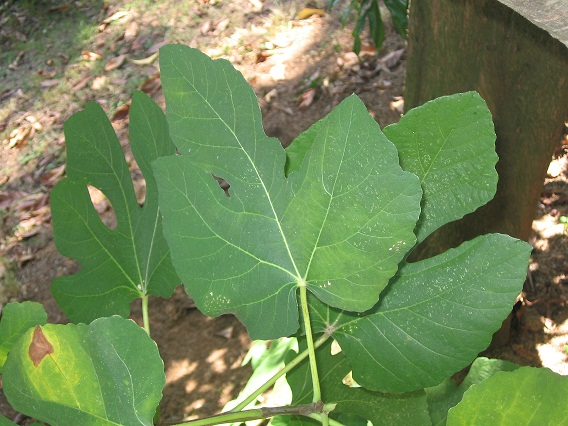
\includegraphics[width=100mm]{leaves.jpg}
	\caption{Caption of the image}
	\label{leave}
\end{center}
\end{figure}

\subsection{Handling bibliography}

Finally, let's find out how a nice bibliography is created. First, check the bibliography styles. A bibliography style tells the document how the references and the list of resources will look like. Currently there exists one style named "alphadin.bst".

In order to set the style do a \textbf{\textbackslash bibliographystyle\{alphadin\}} where "alphadin" (without the ending ".bst") sets the style. If you want to place the bibliography in your text then simply do \textbf{\textbackslash bibliography\{document\}}.

At the time you've created a bibliography (actually, it is created automatically when you create a new project) you can edit its entries by pressing the "Bibliography" button. You can come back here if you press it again. Now that you've entered all your books and articles in the bibliography simply do a \textbf{\textbackslash cite\{refname1\}} where "refname1" specifies the resource you want to cite.

A test: \cite{referenceName1} says that it is a good idea to use LaTeX.

% Create the bibliography right after the text
\bibliographystyle{alphadin}
\bibliography{document}

\end{document}
% All lines that begin with an '%' are comments and won't be displayed in the resulting document1main-branch222

% \documentclass{...} specifies the class of the document. The most common ones are 'book', 'report', 'article' and 'letter'
\documentclass{article}

% Allow the usage of umlauts and other non-ASCII characters
\usepackage[utf8]{inputenc}
% Allow the usage of graphics (.jpg, .png, etc.) in the document
\usepackage{graphicx}
% Allow the change of line spacing
\usepackage{setspace}

% Set line spacing to 1.5xxxneu
\onehalfspacing

% Start the document
\begin{document}

% Show the titlepage (see in 'Documents' below: titlepage.tex)
% Begin a new titlepage. Titlepages have special settings like the absence of page numbers.222
\begin{titlepage}

% Set the text of the page to right-aligned until \end{flushright}
\begin{flushright}

% Set the space between right page border and text to 2.5cm
\rightskip=-2.5cm

% Show an image at this position

\includegraphics[width=50mm]{logo_dark.png}

% Skip a little space
\bigskip
\bigskip
\bigskip
\bigskip

% Create a title for the document and write it in bold font
\LARGE{\textbf{Brief LaTeX Tutorial}}
% Again, do a line break
\linebreak
% Create a subtitle
\large{For LaTeX Beginners}

% Skip some space
\bigskip
\bigskip
\bigskip
\bigskip
\bigskip

% Write in very large letters
\LARGE{verbosus.com}
% Do a line break right after the \LARGE{...} text
\linebreak
% Write in large letters
\large{Free webservices and apps}

% Skip some space
\bigskip
\bigskip
\bigskip
\bigskip
\bigskip
\bigskip

\large{Documentation}

% Skip some space
\bigskip

\normalsize{Vienna, \the\month}

% Skip some space
\bigskip
\bigskip
\bigskip
\bigskip
\bigskip
\bigskip
\bigskip
\bigskip
\bigskip
\bigskip
\bigskip
\bigskip
\bigskip

% Provide some author information
\normalsize{Author:}
\linebreak
\large{Daniel Kuster, MSc}

% End right-alignment at this point
\end{flushright}
% End the title page
\end{titlepage}


% Create a new 1st level heading
\section{First level}

This is the text of the first chapter. If you want to create a subchapter then simply do \textbf{\textbackslash subsection\{Title of first subchapter\}}. If you want to move on to the next chapter then do \textbf{\textbackslash section\{Title of second chapter\}}.

% Create a new 2nd level heading
\subsection{Second level}

Here comes the text of the subsection of the first chapter. Now let's try to insert an image. Currently there exists one image with the name "leaves.jpg" which will be displayed at the current position. This can be changed by changing the [h] (stands for "here", place it at the current position if possible) to a [t] (stands for "top", place it at the beginning of a page if possible), [b] (stands for "bottom", place it at the bottom of a page if possible) or [p] (stands for "float page", place it on a separate page with other floating objects).

The image we've just inserted can be referenced by writing \textbf{\textbackslash ref\{leave\}}. As you can see the figure \ref{leave} shows some leaves.

\subsection{Handling other resource types}

There exist other very useful elements which can be inserted such as tables, itemized lists or description lists. You can try them by simply clicking on the small icons in the editor.

\begin{figure}[htp]
\begin{center}
	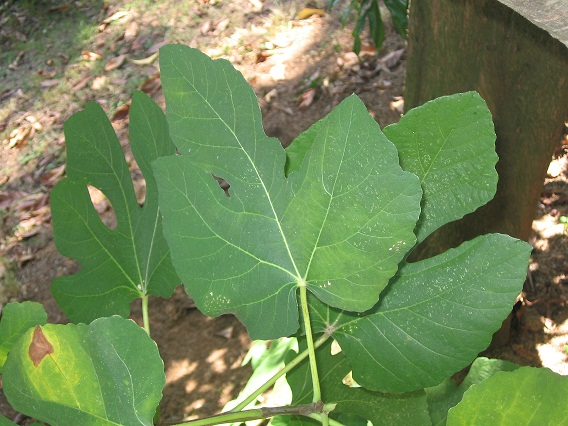
\includegraphics[width=100mm]{leaves.jpg}
	\caption{Caption of the image}
	\label{leave}
\end{center}
\end{figure}

\subsection{Handling bibliography}

Finally, let's find out how a nice bibliography is created. First, check the bibliography styles. A bibliography style tells the document how the references and the list of resources will look like. Currently there exists one style named "alphadin.bst".

In order to set the style do a \textbf{\textbackslash bibliographystyle\{alphadin\}} where "alphadin" (without the ending ".bst") sets the style. If you want to place the bibliography in your text then simply do \textbf{\textbackslash bibliography\{document\}}.

At the time you've created a bibliography (actually, it is created automatically when you create a new project) you can edit its entries by pressing the "Bibliography" button. You can come back here if you press it again. Now that you've entered all your books and articles in the bibliography simply do a \textbf{\textbackslash cite\{refname1\}} where "refname1" specifies the resource you want to cite.

A test: \cite{referenceName1} says that it is a good idea to use LaTeX.

% Create the bibliography right after the text
\bibliographystyle{alphadin}
\bibliography{document}

\end{document}
% All lines that begin with an '%' are comments and won't be displayed in the resulting document1main-branch222

% \documentclass{...} specifies the class of the document. The most common ones are 'book', 'report', 'article' and 'letter'
\documentclass{article}

% Allow the usage of umlauts and other non-ASCII characters
\usepackage[utf8]{inputenc}
% Allow the usage of graphics (.jpg, .png, etc.) in the document
\usepackage{graphicx}
% Allow the change of line spacing
\usepackage{setspace}

% Set line spacing to 1.5xxxneu
\onehalfspacing

% Start the document
\begin{document}

% Show the titlepage (see in 'Documents' below: titlepage.tex)
% Begin a new titlepage. Titlepages have special settings like the absence of page numbers.222
\begin{titlepage}

% Set the text of the page to right-aligned until \end{flushright}
\begin{flushright}

% Set the space between right page border and text to 2.5cm
\rightskip=-2.5cm

% Show an image at this position

\includegraphics[width=50mm]{logo_dark.png}

% Skip a little space
\bigskip
\bigskip
\bigskip
\bigskip

% Create a title for the document and write it in bold font
\LARGE{\textbf{Brief LaTeX Tutorial}}
% Again, do a line break
\linebreak
% Create a subtitle
\large{For LaTeX Beginners}

% Skip some space
\bigskip
\bigskip
\bigskip
\bigskip
\bigskip

% Write in very large letters
\LARGE{verbosus.com}
% Do a line break right after the \LARGE{...} text
\linebreak
% Write in large letters
\large{Free webservices and apps}

% Skip some space
\bigskip
\bigskip
\bigskip
\bigskip
\bigskip
\bigskip

\large{Documentation}

% Skip some space
\bigskip

\normalsize{Vienna, \the\month}

% Skip some space
\bigskip
\bigskip
\bigskip
\bigskip
\bigskip
\bigskip
\bigskip
\bigskip
\bigskip
\bigskip
\bigskip
\bigskip
\bigskip

% Provide some author information
\normalsize{Author:}
\linebreak
\large{Daniel Kuster, MSc}

% End right-alignment at this point
\end{flushright}
% End the title page
\end{titlepage}


% Create a new 1st level heading
\section{First level}

This is the text of the first chapter. If you want to create a subchapter then simply do \textbf{\textbackslash subsection\{Title of first subchapter\}}. If you want to move on to the next chapter then do \textbf{\textbackslash section\{Title of second chapter\}}.

% Create a new 2nd level heading
\subsection{Second level}

Here comes the text of the subsection of the first chapter. Now let's try to insert an image. Currently there exists one image with the name "leaves.jpg" which will be displayed at the current position. This can be changed by changing the [h] (stands for "here", place it at the current position if possible) to a [t] (stands for "top", place it at the beginning of a page if possible), [b] (stands for "bottom", place it at the bottom of a page if possible) or [p] (stands for "float page", place it on a separate page with other floating objects).

The image we've just inserted can be referenced by writing \textbf{\textbackslash ref\{leave\}}. As you can see the figure \ref{leave} shows some leaves.

\subsection{Handling other resource types}

There exist other very useful elements which can be inserted such as tables, itemized lists or description lists. You can try them by simply clicking on the small icons in the editor.

\begin{figure}[htp]
\begin{center}
	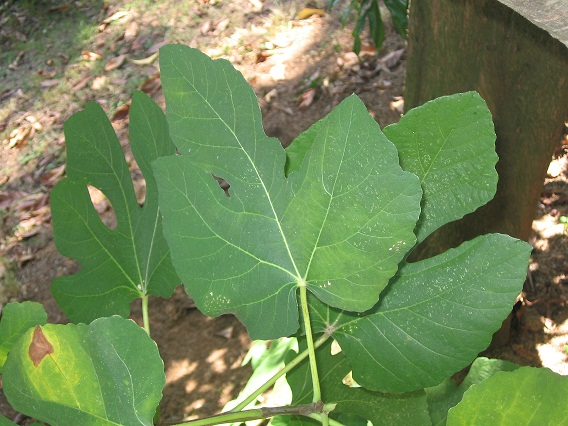
\includegraphics[width=100mm]{leaves.jpg}
	\caption{Caption of the image}
	\label{leave}
\end{center}
\end{figure}

\subsection{Handling bibliography}

Finally, let's find out how a nice bibliography is created. First, check the bibliography styles. A bibliography style tells the document how the references and the list of resources will look like. Currently there exists one style named "alphadin.bst".

In order to set the style do a \textbf{\textbackslash bibliographystyle\{alphadin\}} where "alphadin" (without the ending ".bst") sets the style. If you want to place the bibliography in your text then simply do \textbf{\textbackslash bibliography\{document\}}.

At the time you've created a bibliography (actually, it is created automatically when you create a new project) you can edit its entries by pressing the "Bibliography" button. You can come back here if you press it again. Now that you've entered all your books and articles in the bibliography simply do a \textbf{\textbackslash cite\{refname1\}} where "refname1" specifies the resource you want to cite.

A test: \cite{referenceName1} says that it is a good idea to use LaTeX.

% Create the bibliography right after the text
\bibliographystyle{alphadin}
\bibliography{document}

\end{document}
% All lines that begin with an '%' are comments and won't be displayed in the resulting document1main-branch222

% \documentclass{...} specifies the class of the document. The most common ones are 'book', 'report', 'article' and 'letter'
\documentclass{article}

% Allow the usage of umlauts and other non-ASCII characters
\usepackage[utf8]{inputenc}
% Allow the usage of graphics (.jpg, .png, etc.) in the document
\usepackage{graphicx}
% Allow the change of line spacing
\usepackage{setspace}

% Set line spacing to 1.5xxxneu
\onehalfspacing

% Start the document
\begin{document}

% Show the titlepage (see in 'Documents' below: titlepage.tex)
% Begin a new titlepage. Titlepages have special settings like the absence of page numbers.222
\begin{titlepage}

% Set the text of the page to right-aligned until \end{flushright}
\begin{flushright}

% Set the space between right page border and text to 2.5cm
\rightskip=-2.5cm

% Show an image at this position

\includegraphics[width=50mm]{logo_dark.png}

% Skip a little space
\bigskip
\bigskip
\bigskip
\bigskip

% Create a title for the document and write it in bold font
\LARGE{\textbf{Brief LaTeX Tutorial}}
% Again, do a line break
\linebreak
% Create a subtitle
\large{For LaTeX Beginners}

% Skip some space
\bigskip
\bigskip
\bigskip
\bigskip
\bigskip

% Write in very large letters
\LARGE{verbosus.com}
% Do a line break right after the \LARGE{...} text
\linebreak
% Write in large letters
\large{Free webservices and apps}

% Skip some space
\bigskip
\bigskip
\bigskip
\bigskip
\bigskip
\bigskip

\large{Documentation}

% Skip some space
\bigskip

\normalsize{Vienna, \the\month}

% Skip some space
\bigskip
\bigskip
\bigskip
\bigskip
\bigskip
\bigskip
\bigskip
\bigskip
\bigskip
\bigskip
\bigskip
\bigskip
\bigskip

% Provide some author information
\normalsize{Author:}
\linebreak
\large{Daniel Kuster, MSc}

% End right-alignment at this point
\end{flushright}
% End the title page
\end{titlepage}


% Create a new 1st level heading
\section{First level}

This is the text of the first chapter. If you want to create a subchapter then simply do \textbf{\textbackslash subsection\{Title of first subchapter\}}. If you want to move on to the next chapter then do \textbf{\textbackslash section\{Title of second chapter\}}.

% Create a new 2nd level heading
\subsection{Second level}

Here comes the text of the subsection of the first chapter. Now let's try to insert an image. Currently there exists one image with the name "leaves.jpg" which will be displayed at the current position. This can be changed by changing the [h] (stands for "here", place it at the current position if possible) to a [t] (stands for "top", place it at the beginning of a page if possible), [b] (stands for "bottom", place it at the bottom of a page if possible) or [p] (stands for "float page", place it on a separate page with other floating objects).

The image we've just inserted can be referenced by writing \textbf{\textbackslash ref\{leave\}}. As you can see the figure \ref{leave} shows some leaves.

\subsection{Handling other resource types}

There exist other very useful elements which can be inserted such as tables, itemized lists or description lists. You can try them by simply clicking on the small icons in the editor.

\begin{figure}[htp]
\begin{center}
	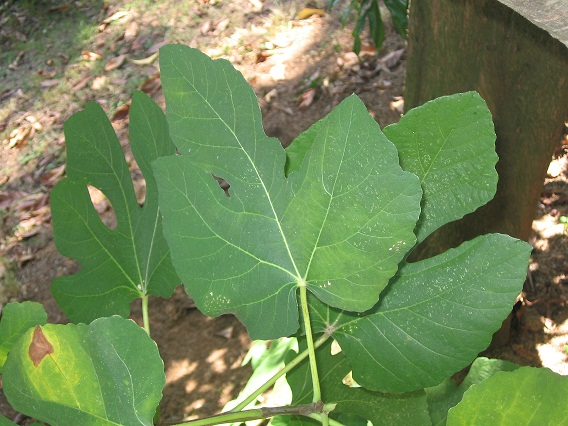
\includegraphics[width=100mm]{leaves.jpg}
	\caption{Caption of the image}
	\label{leave}
\end{center}
\end{figure}

\subsection{Handling bibliography}

Finally, let's find out how a nice bibliography is created. First, check the bibliography styles. A bibliography style tells the document how the references and the list of resources will look like. Currently there exists one style named "alphadin.bst".

In order to set the style do a \textbf{\textbackslash bibliographystyle\{alphadin\}} where "alphadin" (without the ending ".bst") sets the style. If you want to place the bibliography in your text then simply do \textbf{\textbackslash bibliography\{document\}}.

At the time you've created a bibliography (actually, it is created automatically when you create a new project) you can edit its entries by pressing the "Bibliography" button. You can come back here if you press it again. Now that you've entered all your books and articles in the bibliography simply do a \textbf{\textbackslash cite\{refname1\}} where "refname1" specifies the resource you want to cite.

A test: \cite{referenceName1} says that it is a good idea to use LaTeX.

% Create the bibliography right after the text
\bibliographystyle{alphadin}
\bibliography{document}

\end{document}
% All lines that begin with an '%' are comments and won't be displayed in the resulting document1main-branch222

% \documentclass{...} specifies the class of the document. The most common ones are 'book', 'report', 'article' and 'letter'
\documentclass{article}

% Allow the usage of umlauts and other non-ASCII characters
\usepackage[utf8]{inputenc}
% Allow the usage of graphics (.jpg, .png, etc.) in the document
\usepackage{graphicx}
% Allow the change of line spacing
\usepackage{setspace}

% Set line spacing to 1.5xxxneu
\onehalfspacing

% Start the document
\begin{document}

% Show the titlepage (see in 'Documents' below: titlepage.tex)
% Begin a new titlepage. Titlepages have special settings like the absence of page numbers.222
\begin{titlepage}

% Set the text of the page to right-aligned until \end{flushright}
\begin{flushright}

% Set the space between right page border and text to 2.5cm
\rightskip=-2.5cm

% Show an image at this position

\includegraphics[width=50mm]{logo_dark.png}

% Skip a little space
\bigskip
\bigskip
\bigskip
\bigskip

% Create a title for the document and write it in bold font
\LARGE{\textbf{Brief LaTeX Tutorial}}
% Again, do a line break
\linebreak
% Create a subtitle
\large{For LaTeX Beginners}

% Skip some space
\bigskip
\bigskip
\bigskip
\bigskip
\bigskip

% Write in very large letters
\LARGE{verbosus.com}
% Do a line break right after the \LARGE{...} text
\linebreak
% Write in large letters
\large{Free webservices and apps}

% Skip some space
\bigskip
\bigskip
\bigskip
\bigskip
\bigskip
\bigskip

\large{Documentation}

% Skip some space
\bigskip

\normalsize{Vienna, \the\month}

% Skip some space
\bigskip
\bigskip
\bigskip
\bigskip
\bigskip
\bigskip
\bigskip
\bigskip
\bigskip
\bigskip
\bigskip
\bigskip
\bigskip

% Provide some author information
\normalsize{Author:}
\linebreak
\large{Daniel Kuster, MSc}

% End right-alignment at this point
\end{flushright}
% End the title page
\end{titlepage}


% Create a new 1st level heading
\section{First level}

This is the text of the first chapter. If you want to create a subchapter then simply do \textbf{\textbackslash subsection\{Title of first subchapter\}}. If you want to move on to the next chapter then do \textbf{\textbackslash section\{Title of second chapter\}}.

% Create a new 2nd level heading
\subsection{Second level}

Here comes the text of the subsection of the first chapter. Now let's try to insert an image. Currently there exists one image with the name "leaves.jpg" which will be displayed at the current position. This can be changed by changing the [h] (stands for "here", place it at the current position if possible) to a [t] (stands for "top", place it at the beginning of a page if possible), [b] (stands for "bottom", place it at the bottom of a page if possible) or [p] (stands for "float page", place it on a separate page with other floating objects).

The image we've just inserted can be referenced by writing \textbf{\textbackslash ref\{leave\}}. As you can see the figure \ref{leave} shows some leaves.

\subsection{Handling other resource types}

There exist other very useful elements which can be inserted such as tables, itemized lists or description lists. You can try them by simply clicking on the small icons in the editor.

\begin{figure}[htp]
\begin{center}
	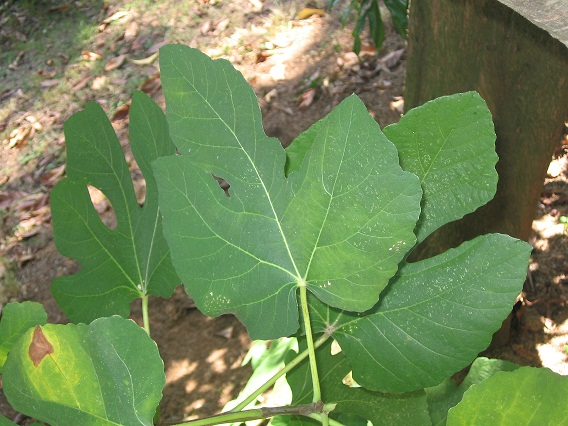
\includegraphics[width=100mm]{leaves.jpg}
	\caption{Caption of the image}
	\label{leave}
\end{center}
\end{figure}

\subsection{Handling bibliography}

Finally, let's find out how a nice bibliography is created. First, check the bibliography styles. A bibliography style tells the document how the references and the list of resources will look like. Currently there exists one style named "alphadin.bst".

In order to set the style do a \textbf{\textbackslash bibliographystyle\{alphadin\}} where "alphadin" (without the ending ".bst") sets the style. If you want to place the bibliography in your text then simply do \textbf{\textbackslash bibliography\{document\}}.

At the time you've created a bibliography (actually, it is created automatically when you create a new project) you can edit its entries by pressing the "Bibliography" button. You can come back here if you press it again. Now that you've entered all your books and articles in the bibliography simply do a \textbf{\textbackslash cite\{refname1\}} where "refname1" specifies the resource you want to cite.

A test: \cite{referenceName1} says that it is a good idea to use LaTeX.

% Create the bibliography right after the text
\bibliographystyle{alphadin}
\bibliography{document}

\end{document}
% All lines that begin with an '%' are comments and won't be displayed in the resulting document1main-branch222

% \documentclass{...} specifies the class of the document. The most common ones are 'book', 'report', 'article' and 'letter'
\documentclass{article}

% Allow the usage of umlauts and other non-ASCII characters
\usepackage[utf8]{inputenc}
% Allow the usage of graphics (.jpg, .png, etc.) in the document
\usepackage{graphicx}
% Allow the change of line spacing
\usepackage{setspace}

% Set line spacing to 1.5xxxneu
\onehalfspacing

% Start the document
\begin{document}

% Show the titlepage (see in 'Documents' below: titlepage.tex)
% Begin a new titlepage. Titlepages have special settings like the absence of page numbers.222
\begin{titlepage}

% Set the text of the page to right-aligned until \end{flushright}
\begin{flushright}

% Set the space between right page border and text to 2.5cm
\rightskip=-2.5cm

% Show an image at this position

\includegraphics[width=50mm]{logo_dark.png}

% Skip a little space
\bigskip
\bigskip
\bigskip
\bigskip

% Create a title for the document and write it in bold font
\LARGE{\textbf{Brief LaTeX Tutorial}}
% Again, do a line break
\linebreak
% Create a subtitle
\large{For LaTeX Beginners}

% Skip some space
\bigskip
\bigskip
\bigskip
\bigskip
\bigskip

% Write in very large letters
\LARGE{verbosus.com}
% Do a line break right after the \LARGE{...} text
\linebreak
% Write in large letters
\large{Free webservices and apps}

% Skip some space
\bigskip
\bigskip
\bigskip
\bigskip
\bigskip
\bigskip

\large{Documentation}

% Skip some space
\bigskip

\normalsize{Vienna, \the\month}

% Skip some space
\bigskip
\bigskip
\bigskip
\bigskip
\bigskip
\bigskip
\bigskip
\bigskip
\bigskip
\bigskip
\bigskip
\bigskip
\bigskip

% Provide some author information
\normalsize{Author:}
\linebreak
\large{Daniel Kuster, MSc}

% End right-alignment at this point
\end{flushright}
% End the title page
\end{titlepage}


% Create a new 1st level heading
\section{First level}

This is the text of the first chapter. If you want to create a subchapter then simply do \textbf{\textbackslash subsection\{Title of first subchapter\}}. If you want to move on to the next chapter then do \textbf{\textbackslash section\{Title of second chapter\}}.

% Create a new 2nd level heading
\subsection{Second level}

Here comes the text of the subsection of the first chapter. Now let's try to insert an image. Currently there exists one image with the name "leaves.jpg" which will be displayed at the current position. This can be changed by changing the [h] (stands for "here", place it at the current position if possible) to a [t] (stands for "top", place it at the beginning of a page if possible), [b] (stands for "bottom", place it at the bottom of a page if possible) or [p] (stands for "float page", place it on a separate page with other floating objects).

The image we've just inserted can be referenced by writing \textbf{\textbackslash ref\{leave\}}. As you can see the figure \ref{leave} shows some leaves.

\subsection{Handling other resource types}

There exist other very useful elements which can be inserted such as tables, itemized lists or description lists. You can try them by simply clicking on the small icons in the editor.

\begin{figure}[htp]
\begin{center}
	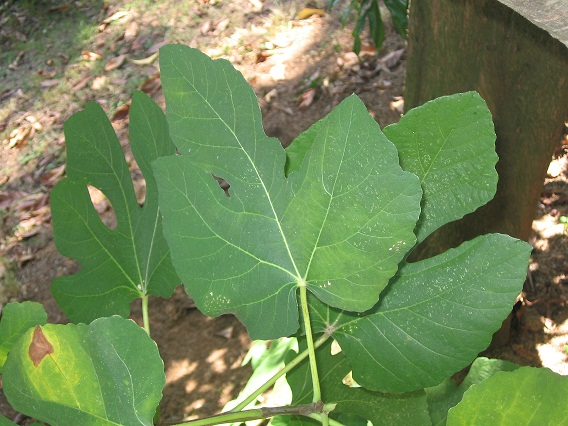
\includegraphics[width=100mm]{leaves.jpg}
	\caption{Caption of the image}
	\label{leave}
\end{center}
\end{figure}

\subsection{Handling bibliography}

Finally, let's find out how a nice bibliography is created. First, check the bibliography styles. A bibliography style tells the document how the references and the list of resources will look like. Currently there exists one style named "alphadin.bst".

In order to set the style do a \textbf{\textbackslash bibliographystyle\{alphadin\}} where "alphadin" (without the ending ".bst") sets the style. If you want to place the bibliography in your text then simply do \textbf{\textbackslash bibliography\{document\}}.

At the time you've created a bibliography (actually, it is created automatically when you create a new project) you can edit its entries by pressing the "Bibliography" button. You can come back here if you press it again. Now that you've entered all your books and articles in the bibliography simply do a \textbf{\textbackslash cite\{refname1\}} where "refname1" specifies the resource you want to cite.

A test: \cite{referenceName1} says that it is a good idea to use LaTeX.

% Create the bibliography right after the text
\bibliographystyle{alphadin}
\bibliography{document}

\end{document}
% All lines that begin with an '%' are comments and won't be displayed in the resulting document1main-branch222

% \documentclass{...} specifies the class of the document. The most common ones are 'book', 'report', 'article' and 'letter'
\documentclass{article}

% Allow the usage of umlauts and other non-ASCII characters
\usepackage[utf8]{inputenc}
% Allow the usage of graphics (.jpg, .png, etc.) in the document
\usepackage{graphicx}
% Allow the change of line spacing
\usepackage{setspace}

% Set line spacing to 1.5xxxneu
\onehalfspacing

% Start the document
\begin{document}

% Show the titlepage (see in 'Documents' below: titlepage.tex)
% Begin a new titlepage. Titlepages have special settings like the absence of page numbers.222
\begin{titlepage}

% Set the text of the page to right-aligned until \end{flushright}
\begin{flushright}

% Set the space between right page border and text to 2.5cm
\rightskip=-2.5cm

% Show an image at this position

\includegraphics[width=50mm]{logo_dark.png}

% Skip a little space
\bigskip
\bigskip
\bigskip
\bigskip

% Create a title for the document and write it in bold font
\LARGE{\textbf{Brief LaTeX Tutorial}}
% Again, do a line break
\linebreak
% Create a subtitle
\large{For LaTeX Beginners}

% Skip some space
\bigskip
\bigskip
\bigskip
\bigskip
\bigskip

% Write in very large letters
\LARGE{verbosus.com}
% Do a line break right after the \LARGE{...} text
\linebreak
% Write in large letters
\large{Free webservices and apps}

% Skip some space
\bigskip
\bigskip
\bigskip
\bigskip
\bigskip
\bigskip

\large{Documentation}

% Skip some space
\bigskip

\normalsize{Vienna, \the\month}

% Skip some space
\bigskip
\bigskip
\bigskip
\bigskip
\bigskip
\bigskip
\bigskip
\bigskip
\bigskip
\bigskip
\bigskip
\bigskip
\bigskip

% Provide some author information
\normalsize{Author:}
\linebreak
\large{Daniel Kuster, MSc}

% End right-alignment at this point
\end{flushright}
% End the title page
\end{titlepage}


% Create a new 1st level heading
\section{First level}

This is the text of the first chapter. If you want to create a subchapter then simply do \textbf{\textbackslash subsection\{Title of first subchapter\}}. If you want to move on to the next chapter then do \textbf{\textbackslash section\{Title of second chapter\}}.

% Create a new 2nd level heading
\subsection{Second level}

Here comes the text of the subsection of the first chapter. Now let's try to insert an image. Currently there exists one image with the name "leaves.jpg" which will be displayed at the current position. This can be changed by changing the [h] (stands for "here", place it at the current position if possible) to a [t] (stands for "top", place it at the beginning of a page if possible), [b] (stands for "bottom", place it at the bottom of a page if possible) or [p] (stands for "float page", place it on a separate page with other floating objects).

The image we've just inserted can be referenced by writing \textbf{\textbackslash ref\{leave\}}. As you can see the figure \ref{leave} shows some leaves.

\subsection{Handling other resource types}

There exist other very useful elements which can be inserted such as tables, itemized lists or description lists. You can try them by simply clicking on the small icons in the editor.

\begin{figure}[htp]
\begin{center}
	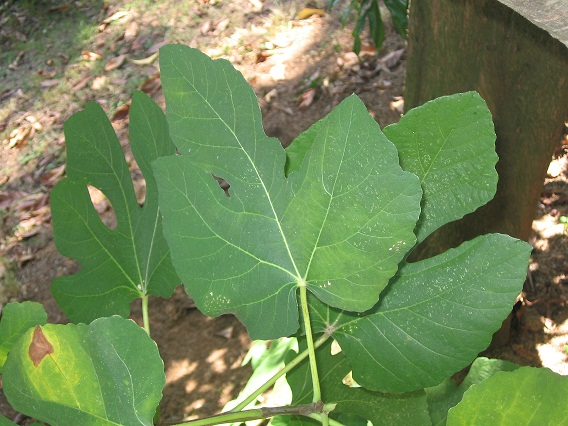
\includegraphics[width=100mm]{leaves.jpg}
	\caption{Caption of the image}
	\label{leave}
\end{center}
\end{figure}

\subsection{Handling bibliography}

Finally, let's find out how a nice bibliography is created. First, check the bibliography styles. A bibliography style tells the document how the references and the list of resources will look like. Currently there exists one style named "alphadin.bst".

In order to set the style do a \textbf{\textbackslash bibliographystyle\{alphadin\}} where "alphadin" (without the ending ".bst") sets the style. If you want to place the bibliography in your text then simply do \textbf{\textbackslash bibliography\{document\}}.

At the time you've created a bibliography (actually, it is created automatically when you create a new project) you can edit its entries by pressing the "Bibliography" button. You can come back here if you press it again. Now that you've entered all your books and articles in the bibliography simply do a \textbf{\textbackslash cite\{refname1\}} where "refname1" specifies the resource you want to cite.

A test: \cite{referenceName1} says that it is a good idea to use LaTeX.

% Create the bibliography right after the text
\bibliographystyle{alphadin}
\bibliography{document}

\end{document}
% All lines that begin with an '%' are comments and won't be displayed in the resulting document1main-branch222

% \documentclass{...} specifies the class of the document. The most common ones are 'book', 'report', 'article' and 'letter'
\documentclass{article}

% Allow the usage of umlauts and other non-ASCII characters
\usepackage[utf8]{inputenc}
% Allow the usage of graphics (.jpg, .png, etc.) in the document
\usepackage{graphicx}
% Allow the change of line spacing
\usepackage{setspace}

% Set line spacing to 1.5xxxneu
\onehalfspacing

% Start the document
\begin{document}

% Show the titlepage (see in 'Documents' below: titlepage.tex)
% Begin a new titlepage. Titlepages have special settings like the absence of page numbers.222
\begin{titlepage}

% Set the text of the page to right-aligned until \end{flushright}
\begin{flushright}

% Set the space between right page border and text to 2.5cm
\rightskip=-2.5cm

% Show an image at this position

\includegraphics[width=50mm]{logo_dark.png}

% Skip a little space
\bigskip
\bigskip
\bigskip
\bigskip

% Create a title for the document and write it in bold font
\LARGE{\textbf{Brief LaTeX Tutorial}}
% Again, do a line break
\linebreak
% Create a subtitle
\large{For LaTeX Beginners}

% Skip some space
\bigskip
\bigskip
\bigskip
\bigskip
\bigskip

% Write in very large letters
\LARGE{verbosus.com}
% Do a line break right after the \LARGE{...} text
\linebreak
% Write in large letters
\large{Free webservices and apps}

% Skip some space
\bigskip
\bigskip
\bigskip
\bigskip
\bigskip
\bigskip

\large{Documentation}

% Skip some space
\bigskip

\normalsize{Vienna, \the\month}

% Skip some space
\bigskip
\bigskip
\bigskip
\bigskip
\bigskip
\bigskip
\bigskip
\bigskip
\bigskip
\bigskip
\bigskip
\bigskip
\bigskip

% Provide some author information
\normalsize{Author:}
\linebreak
\large{Daniel Kuster, MSc}

% End right-alignment at this point
\end{flushright}
% End the title page
\end{titlepage}


% Create a new 1st level heading
\section{First level}

This is the text of the first chapter. If you want to create a subchapter then simply do \textbf{\textbackslash subsection\{Title of first subchapter\}}. If you want to move on to the next chapter then do \textbf{\textbackslash section\{Title of second chapter\}}.

% Create a new 2nd level heading
\subsection{Second level}

Here comes the text of the subsection of the first chapter. Now let's try to insert an image. Currently there exists one image with the name "leaves.jpg" which will be displayed at the current position. This can be changed by changing the [h] (stands for "here", place it at the current position if possible) to a [t] (stands for "top", place it at the beginning of a page if possible), [b] (stands for "bottom", place it at the bottom of a page if possible) or [p] (stands for "float page", place it on a separate page with other floating objects).

The image we've just inserted can be referenced by writing \textbf{\textbackslash ref\{leave\}}. As you can see the figure \ref{leave} shows some leaves.

\subsection{Handling other resource types}

There exist other very useful elements which can be inserted such as tables, itemized lists or description lists. You can try them by simply clicking on the small icons in the editor.

\begin{figure}[htp]
\begin{center}
	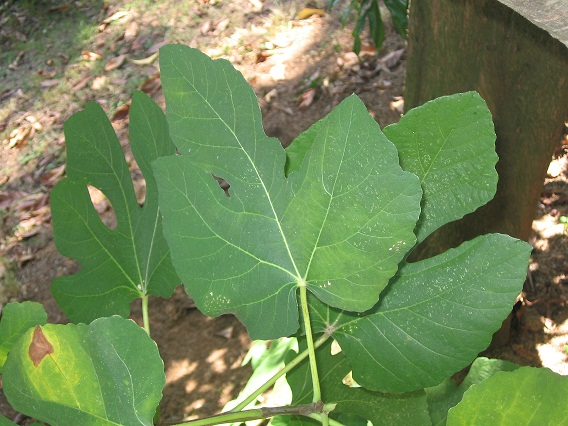
\includegraphics[width=100mm]{leaves.jpg}
	\caption{Caption of the image}
	\label{leave}
\end{center}
\end{figure}

\subsection{Handling bibliography}

Finally, let's find out how a nice bibliography is created. First, check the bibliography styles. A bibliography style tells the document how the references and the list of resources will look like. Currently there exists one style named "alphadin.bst".

In order to set the style do a \textbf{\textbackslash bibliographystyle\{alphadin\}} where "alphadin" (without the ending ".bst") sets the style. If you want to place the bibliography in your text then simply do \textbf{\textbackslash bibliography\{document\}}.

At the time you've created a bibliography (actually, it is created automatically when you create a new project) you can edit its entries by pressing the "Bibliography" button. You can come back here if you press it again. Now that you've entered all your books and articles in the bibliography simply do a \textbf{\textbackslash cite\{refname1\}} where "refname1" specifies the resource you want to cite.

A test: \cite{referenceName1} says that it is a good idea to use LaTeX.

% Create the bibliography right after the text
\bibliographystyle{alphadin}
\bibliography{document}

\end{document}
% All lines that begin with an '%' are comments and won't be displayed in the resulting document1main-branch222

% \documentclass{...} specifies the class of the document. The most common ones are 'book', 'report', 'article' and 'letter'
\documentclass{article}

% Allow the usage of umlauts and other non-ASCII characters
\usepackage[utf8]{inputenc}
% Allow the usage of graphics (.jpg, .png, etc.) in the document
\usepackage{graphicx}
% Allow the change of line spacing
\usepackage{setspace}

% Set line spacing to 1.5xxxneu
\onehalfspacing

% Start the document
\begin{document}

% Show the titlepage (see in 'Documents' below: titlepage.tex)
% Begin a new titlepage. Titlepages have special settings like the absence of page numbers.222
\begin{titlepage}

% Set the text of the page to right-aligned until \end{flushright}
\begin{flushright}

% Set the space between right page border and text to 2.5cm
\rightskip=-2.5cm

% Show an image at this position

\includegraphics[width=50mm]{logo_dark.png}

% Skip a little space
\bigskip
\bigskip
\bigskip
\bigskip

% Create a title for the document and write it in bold font
\LARGE{\textbf{Brief LaTeX Tutorial}}
% Again, do a line break
\linebreak
% Create a subtitle
\large{For LaTeX Beginners}

% Skip some space
\bigskip
\bigskip
\bigskip
\bigskip
\bigskip

% Write in very large letters
\LARGE{verbosus.com}
% Do a line break right after the \LARGE{...} text
\linebreak
% Write in large letters
\large{Free webservices and apps}

% Skip some space
\bigskip
\bigskip
\bigskip
\bigskip
\bigskip
\bigskip

\large{Documentation}

% Skip some space
\bigskip

\normalsize{Vienna, \the\month}

% Skip some space
\bigskip
\bigskip
\bigskip
\bigskip
\bigskip
\bigskip
\bigskip
\bigskip
\bigskip
\bigskip
\bigskip
\bigskip
\bigskip

% Provide some author information
\normalsize{Author:}
\linebreak
\large{Daniel Kuster, MSc}

% End right-alignment at this point
\end{flushright}
% End the title page
\end{titlepage}


% Create a new 1st level heading
\section{First level}

This is the text of the first chapter. If you want to create a subchapter then simply do \textbf{\textbackslash subsection\{Title of first subchapter\}}. If you want to move on to the next chapter then do \textbf{\textbackslash section\{Title of second chapter\}}.

% Create a new 2nd level heading
\subsection{Second level}

Here comes the text of the subsection of the first chapter. Now let's try to insert an image. Currently there exists one image with the name "leaves.jpg" which will be displayed at the current position. This can be changed by changing the [h] (stands for "here", place it at the current position if possible) to a [t] (stands for "top", place it at the beginning of a page if possible), [b] (stands for "bottom", place it at the bottom of a page if possible) or [p] (stands for "float page", place it on a separate page with other floating objects).

The image we've just inserted can be referenced by writing \textbf{\textbackslash ref\{leave\}}. As you can see the figure \ref{leave} shows some leaves.

\subsection{Handling other resource types}

There exist other very useful elements which can be inserted such as tables, itemized lists or description lists. You can try them by simply clicking on the small icons in the editor.

\begin{figure}[htp]
\begin{center}
	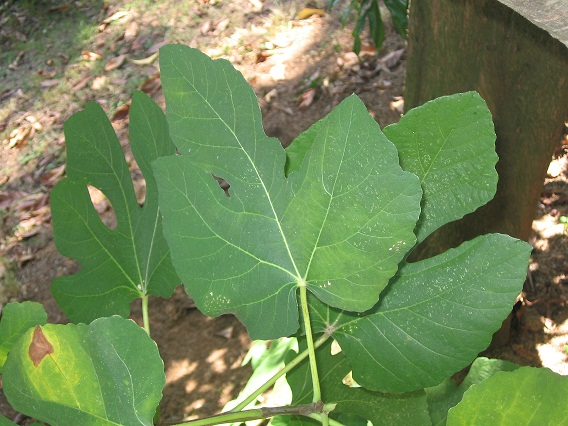
\includegraphics[width=100mm]{leaves.jpg}
	\caption{Caption of the image}
	\label{leave}
\end{center}
\end{figure}

\subsection{Handling bibliography}

Finally, let's find out how a nice bibliography is created. First, check the bibliography styles. A bibliography style tells the document how the references and the list of resources will look like. Currently there exists one style named "alphadin.bst".

In order to set the style do a \textbf{\textbackslash bibliographystyle\{alphadin\}} where "alphadin" (without the ending ".bst") sets the style. If you want to place the bibliography in your text then simply do \textbf{\textbackslash bibliography\{document\}}.

At the time you've created a bibliography (actually, it is created automatically when you create a new project) you can edit its entries by pressing the "Bibliography" button. You can come back here if you press it again. Now that you've entered all your books and articles in the bibliography simply do a \textbf{\textbackslash cite\{refname1\}} where "refname1" specifies the resource you want to cite.

A test: \cite{referenceName1} says that it is a good idea to use LaTeX.

% Create the bibliography right after the text
\bibliographystyle{alphadin}
\bibliography{document}

\end{document}
% All lines that begin with an '%' are comments and won't be displayed in the resulting document1main-branch222

% \documentclass{...} specifies the class of the document. The most common ones are 'book', 'report', 'article' and 'letter'
\documentclass{article}

% Allow the usage of umlauts and other non-ASCII characters
\usepackage[utf8]{inputenc}
% Allow the usage of graphics (.jpg, .png, etc.) in the document
\usepackage{graphicx}
% Allow the change of line spacing
\usepackage{setspace}

% Set line spacing to 1.5xxxneu
\onehalfspacing

% Start the document
\begin{document}

% Show the titlepage (see in 'Documents' below: titlepage.tex)
% Begin a new titlepage. Titlepages have special settings like the absence of page numbers.222
\begin{titlepage}

% Set the text of the page to right-aligned until \end{flushright}
\begin{flushright}

% Set the space between right page border and text to 2.5cm
\rightskip=-2.5cm

% Show an image at this position

\includegraphics[width=50mm]{logo_dark.png}

% Skip a little space
\bigskip
\bigskip
\bigskip
\bigskip

% Create a title for the document and write it in bold font
\LARGE{\textbf{Brief LaTeX Tutorial}}
% Again, do a line break
\linebreak
% Create a subtitle
\large{For LaTeX Beginners}

% Skip some space
\bigskip
\bigskip
\bigskip
\bigskip
\bigskip

% Write in very large letters
\LARGE{verbosus.com}
% Do a line break right after the \LARGE{...} text
\linebreak
% Write in large letters
\large{Free webservices and apps}

% Skip some space
\bigskip
\bigskip
\bigskip
\bigskip
\bigskip
\bigskip

\large{Documentation}

% Skip some space
\bigskip

\normalsize{Vienna, \the\month}

% Skip some space
\bigskip
\bigskip
\bigskip
\bigskip
\bigskip
\bigskip
\bigskip
\bigskip
\bigskip
\bigskip
\bigskip
\bigskip
\bigskip

% Provide some author information
\normalsize{Author:}
\linebreak
\large{Daniel Kuster, MSc}

% End right-alignment at this point
\end{flushright}
% End the title page
\end{titlepage}


% Create a new 1st level heading
\section{First level}

This is the text of the first chapter. If you want to create a subchapter then simply do \textbf{\textbackslash subsection\{Title of first subchapter\}}. If you want to move on to the next chapter then do \textbf{\textbackslash section\{Title of second chapter\}}.

% Create a new 2nd level heading
\subsection{Second level}

Here comes the text of the subsection of the first chapter. Now let's try to insert an image. Currently there exists one image with the name "leaves.jpg" which will be displayed at the current position. This can be changed by changing the [h] (stands for "here", place it at the current position if possible) to a [t] (stands for "top", place it at the beginning of a page if possible), [b] (stands for "bottom", place it at the bottom of a page if possible) or [p] (stands for "float page", place it on a separate page with other floating objects).

The image we've just inserted can be referenced by writing \textbf{\textbackslash ref\{leave\}}. As you can see the figure \ref{leave} shows some leaves.

\subsection{Handling other resource types}

There exist other very useful elements which can be inserted such as tables, itemized lists or description lists. You can try them by simply clicking on the small icons in the editor.

\begin{figure}[htp]
\begin{center}
	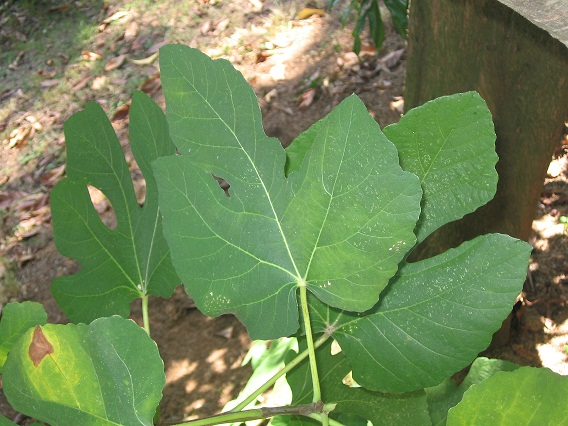
\includegraphics[width=100mm]{leaves.jpg}
	\caption{Caption of the image}
	\label{leave}
\end{center}
\end{figure}

\subsection{Handling bibliography}

Finally, let's find out how a nice bibliography is created. First, check the bibliography styles. A bibliography style tells the document how the references and the list of resources will look like. Currently there exists one style named "alphadin.bst".

In order to set the style do a \textbf{\textbackslash bibliographystyle\{alphadin\}} where "alphadin" (without the ending ".bst") sets the style. If you want to place the bibliography in your text then simply do \textbf{\textbackslash bibliography\{document\}}.

At the time you've created a bibliography (actually, it is created automatically when you create a new project) you can edit its entries by pressing the "Bibliography" button. You can come back here if you press it again. Now that you've entered all your books and articles in the bibliography simply do a \textbf{\textbackslash cite\{refname1\}} where "refname1" specifies the resource you want to cite.

A test: \cite{referenceName1} says that it is a good idea to use LaTeX.

% Create the bibliography right after the text
\bibliographystyle{alphadin}
\bibliography{document}

\end{document}
% All lines that begin with an '%' are comments and won't be displayed in the resulting document1main-branch222

% \documentclass{...} specifies the class of the document. The most common ones are 'book', 'report', 'article' and 'letter'
\documentclass{article}

% Allow the usage of umlauts and other non-ASCII characters
\usepackage[utf8]{inputenc}
% Allow the usage of graphics (.jpg, .png, etc.) in the document
\usepackage{graphicx}
% Allow the change of line spacing
\usepackage{setspace}

% Set line spacing to 1.5xxxneu
\onehalfspacing

% Start the document
\begin{document}

% Show the titlepage (see in 'Documents' below: titlepage.tex)
% Begin a new titlepage. Titlepages have special settings like the absence of page numbers.222
\begin{titlepage}

% Set the text of the page to right-aligned until \end{flushright}
\begin{flushright}

% Set the space between right page border and text to 2.5cm
\rightskip=-2.5cm

% Show an image at this position

\includegraphics[width=50mm]{logo_dark.png}

% Skip a little space
\bigskip
\bigskip
\bigskip
\bigskip

% Create a title for the document and write it in bold font
\LARGE{\textbf{Brief LaTeX Tutorial}}
% Again, do a line break
\linebreak
% Create a subtitle
\large{For LaTeX Beginners}

% Skip some space
\bigskip
\bigskip
\bigskip
\bigskip
\bigskip

% Write in very large letters
\LARGE{verbosus.com}
% Do a line break right after the \LARGE{...} text
\linebreak
% Write in large letters
\large{Free webservices and apps}

% Skip some space
\bigskip
\bigskip
\bigskip
\bigskip
\bigskip
\bigskip

\large{Documentation}

% Skip some space
\bigskip

\normalsize{Vienna, \the\month}

% Skip some space
\bigskip
\bigskip
\bigskip
\bigskip
\bigskip
\bigskip
\bigskip
\bigskip
\bigskip
\bigskip
\bigskip
\bigskip
\bigskip

% Provide some author information
\normalsize{Author:}
\linebreak
\large{Daniel Kuster, MSc}

% End right-alignment at this point
\end{flushright}
% End the title page
\end{titlepage}


% Create a new 1st level heading
\section{First level}

This is the text of the first chapter. If you want to create a subchapter then simply do \textbf{\textbackslash subsection\{Title of first subchapter\}}. If you want to move on to the next chapter then do \textbf{\textbackslash section\{Title of second chapter\}}.

% Create a new 2nd level heading
\subsection{Second level}

Here comes the text of the subsection of the first chapter. Now let's try to insert an image. Currently there exists one image with the name "leaves.jpg" which will be displayed at the current position. This can be changed by changing the [h] (stands for "here", place it at the current position if possible) to a [t] (stands for "top", place it at the beginning of a page if possible), [b] (stands for "bottom", place it at the bottom of a page if possible) or [p] (stands for "float page", place it on a separate page with other floating objects).

The image we've just inserted can be referenced by writing \textbf{\textbackslash ref\{leave\}}. As you can see the figure \ref{leave} shows some leaves.

\subsection{Handling other resource types}

There exist other very useful elements which can be inserted such as tables, itemized lists or description lists. You can try them by simply clicking on the small icons in the editor.

\begin{figure}[htp]
\begin{center}
	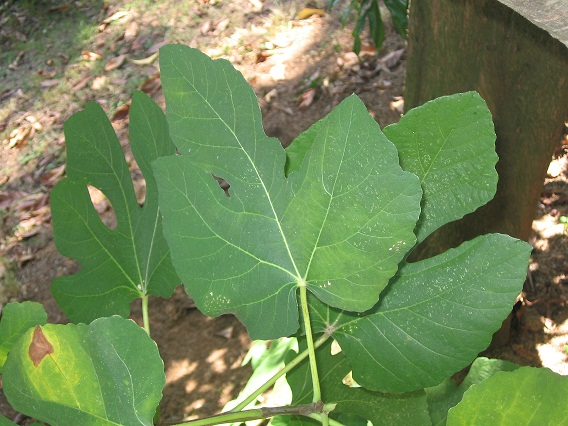
\includegraphics[width=100mm]{leaves.jpg}
	\caption{Caption of the image}
	\label{leave}
\end{center}
\end{figure}

\subsection{Handling bibliography}

Finally, let's find out how a nice bibliography is created. First, check the bibliography styles. A bibliography style tells the document how the references and the list of resources will look like. Currently there exists one style named "alphadin.bst".

In order to set the style do a \textbf{\textbackslash bibliographystyle\{alphadin\}} where "alphadin" (without the ending ".bst") sets the style. If you want to place the bibliography in your text then simply do \textbf{\textbackslash bibliography\{document\}}.

At the time you've created a bibliography (actually, it is created automatically when you create a new project) you can edit its entries by pressing the "Bibliography" button. You can come back here if you press it again. Now that you've entered all your books and articles in the bibliography simply do a \textbf{\textbackslash cite\{refname1\}} where "refname1" specifies the resource you want to cite.

A test: \cite{referenceName1} says that it is a good idea to use LaTeX.

% Create the bibliography right after the text
\bibliographystyle{alphadin}
\bibliography{document}

\end{document}
% All lines that begin with an '%' are comments and won't be displayed in the resulting document1main-branch222

% \documentclass{...} specifies the class of the document. The most common ones are 'book', 'report', 'article' and 'letter'
\documentclass{article}

% Allow the usage of umlauts and other non-ASCII characters
\usepackage[utf8]{inputenc}
% Allow the usage of graphics (.jpg, .png, etc.) in the document
\usepackage{graphicx}
% Allow the change of line spacing
\usepackage{setspace}

% Set line spacing to 1.5xxxneu
\onehalfspacing

% Start the document
\begin{document}

% Show the titlepage (see in 'Documents' below: titlepage.tex)
% Begin a new titlepage. Titlepages have special settings like the absence of page numbers.222
\begin{titlepage}

% Set the text of the page to right-aligned until \end{flushright}
\begin{flushright}

% Set the space between right page border and text to 2.5cm
\rightskip=-2.5cm

% Show an image at this position

\includegraphics[width=50mm]{logo_dark.png}

% Skip a little space
\bigskip
\bigskip
\bigskip
\bigskip

% Create a title for the document and write it in bold font
\LARGE{\textbf{Brief LaTeX Tutorial}}
% Again, do a line break
\linebreak
% Create a subtitle
\large{For LaTeX Beginners}

% Skip some space
\bigskip
\bigskip
\bigskip
\bigskip
\bigskip

% Write in very large letters
\LARGE{verbosus.com}
% Do a line break right after the \LARGE{...} text
\linebreak
% Write in large letters
\large{Free webservices and apps}

% Skip some space
\bigskip
\bigskip
\bigskip
\bigskip
\bigskip
\bigskip

\large{Documentation}

% Skip some space
\bigskip

\normalsize{Vienna, \the\month}

% Skip some space
\bigskip
\bigskip
\bigskip
\bigskip
\bigskip
\bigskip
\bigskip
\bigskip
\bigskip
\bigskip
\bigskip
\bigskip
\bigskip

% Provide some author information
\normalsize{Author:}
\linebreak
\large{Daniel Kuster, MSc}

% End right-alignment at this point
\end{flushright}
% End the title page
\end{titlepage}


% Create a new 1st level heading
\section{First level}

This is the text of the first chapter. If you want to create a subchapter then simply do \textbf{\textbackslash subsection\{Title of first subchapter\}}. If you want to move on to the next chapter then do \textbf{\textbackslash section\{Title of second chapter\}}.

% Create a new 2nd level heading
\subsection{Second level}

Here comes the text of the subsection of the first chapter. Now let's try to insert an image. Currently there exists one image with the name "leaves.jpg" which will be displayed at the current position. This can be changed by changing the [h] (stands for "here", place it at the current position if possible) to a [t] (stands for "top", place it at the beginning of a page if possible), [b] (stands for "bottom", place it at the bottom of a page if possible) or [p] (stands for "float page", place it on a separate page with other floating objects).

The image we've just inserted can be referenced by writing \textbf{\textbackslash ref\{leave\}}. As you can see the figure \ref{leave} shows some leaves.

\subsection{Handling other resource types}

There exist other very useful elements which can be inserted such as tables, itemized lists or description lists. You can try them by simply clicking on the small icons in the editor.

\begin{figure}[htp]
\begin{center}
	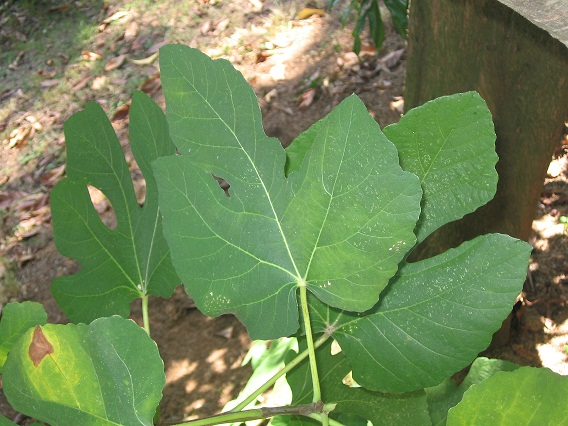
\includegraphics[width=100mm]{leaves.jpg}
	\caption{Caption of the image}
	\label{leave}
\end{center}
\end{figure}

\subsection{Handling bibliography}

Finally, let's find out how a nice bibliography is created. First, check the bibliography styles. A bibliography style tells the document how the references and the list of resources will look like. Currently there exists one style named "alphadin.bst".

In order to set the style do a \textbf{\textbackslash bibliographystyle\{alphadin\}} where "alphadin" (without the ending ".bst") sets the style. If you want to place the bibliography in your text then simply do \textbf{\textbackslash bibliography\{document\}}.

At the time you've created a bibliography (actually, it is created automatically when you create a new project) you can edit its entries by pressing the "Bibliography" button. You can come back here if you press it again. Now that you've entered all your books and articles in the bibliography simply do a \textbf{\textbackslash cite\{refname1\}} where "refname1" specifies the resource you want to cite.

A test: \cite{referenceName1} says that it is a good idea to use LaTeX.

% Create the bibliography right after the text
\bibliographystyle{alphadin}
\bibliography{document}

\end{document}
% All lines that begin with an '%' are comments and won't be displayed in the resulting document1main-branch222

% \documentclass{...} specifies the class of the document. The most common ones are 'book', 'report', 'article' and 'letter'
\documentclass{article}

% Allow the usage of umlauts and other non-ASCII characters
\usepackage[utf8]{inputenc}
% Allow the usage of graphics (.jpg, .png, etc.) in the document
\usepackage{graphicx}
% Allow the change of line spacing
\usepackage{setspace}

% Set line spacing to 1.5xxxneu
\onehalfspacing

% Start the document
\begin{document}

% Show the titlepage (see in 'Documents' below: titlepage.tex)
% Begin a new titlepage. Titlepages have special settings like the absence of page numbers.222
\begin{titlepage}

% Set the text of the page to right-aligned until \end{flushright}
\begin{flushright}

% Set the space between right page border and text to 2.5cm
\rightskip=-2.5cm

% Show an image at this position

\includegraphics[width=50mm]{logo_dark.png}

% Skip a little space
\bigskip
\bigskip
\bigskip
\bigskip

% Create a title for the document and write it in bold font
\LARGE{\textbf{Brief LaTeX Tutorial}}
% Again, do a line break
\linebreak
% Create a subtitle
\large{For LaTeX Beginners}

% Skip some space
\bigskip
\bigskip
\bigskip
\bigskip
\bigskip

% Write in very large letters
\LARGE{verbosus.com}
% Do a line break right after the \LARGE{...} text
\linebreak
% Write in large letters
\large{Free webservices and apps}

% Skip some space
\bigskip
\bigskip
\bigskip
\bigskip
\bigskip
\bigskip

\large{Documentation}

% Skip some space
\bigskip

\normalsize{Vienna, \the\month}

% Skip some space
\bigskip
\bigskip
\bigskip
\bigskip
\bigskip
\bigskip
\bigskip
\bigskip
\bigskip
\bigskip
\bigskip
\bigskip
\bigskip

% Provide some author information
\normalsize{Author:}
\linebreak
\large{Daniel Kuster, MSc}

% End right-alignment at this point
\end{flushright}
% End the title page
\end{titlepage}


% Create a new 1st level heading
\section{First level}

This is the text of the first chapter. If you want to create a subchapter then simply do \textbf{\textbackslash subsection\{Title of first subchapter\}}. If you want to move on to the next chapter then do \textbf{\textbackslash section\{Title of second chapter\}}.

% Create a new 2nd level heading
\subsection{Second level}

Here comes the text of the subsection of the first chapter. Now let's try to insert an image. Currently there exists one image with the name "leaves.jpg" which will be displayed at the current position. This can be changed by changing the [h] (stands for "here", place it at the current position if possible) to a [t] (stands for "top", place it at the beginning of a page if possible), [b] (stands for "bottom", place it at the bottom of a page if possible) or [p] (stands for "float page", place it on a separate page with other floating objects).

The image we've just inserted can be referenced by writing \textbf{\textbackslash ref\{leave\}}. As you can see the figure \ref{leave} shows some leaves.

\subsection{Handling other resource types}

There exist other very useful elements which can be inserted such as tables, itemized lists or description lists. You can try them by simply clicking on the small icons in the editor.

\begin{figure}[htp]
\begin{center}
	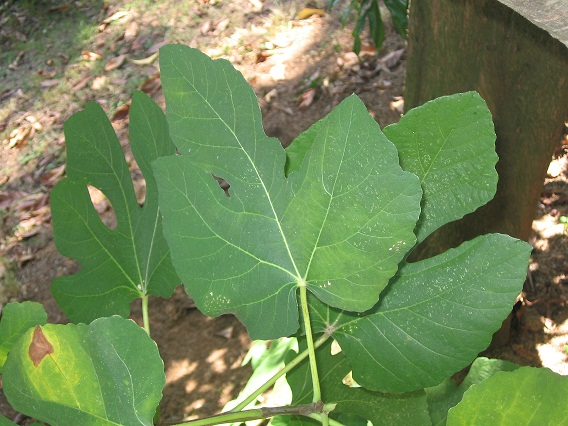
\includegraphics[width=100mm]{leaves.jpg}
	\caption{Caption of the image}
	\label{leave}
\end{center}
\end{figure}

\subsection{Handling bibliography}

Finally, let's find out how a nice bibliography is created. First, check the bibliography styles. A bibliography style tells the document how the references and the list of resources will look like. Currently there exists one style named "alphadin.bst".

In order to set the style do a \textbf{\textbackslash bibliographystyle\{alphadin\}} where "alphadin" (without the ending ".bst") sets the style. If you want to place the bibliography in your text then simply do \textbf{\textbackslash bibliography\{document\}}.

At the time you've created a bibliography (actually, it is created automatically when you create a new project) you can edit its entries by pressing the "Bibliography" button. You can come back here if you press it again. Now that you've entered all your books and articles in the bibliography simply do a \textbf{\textbackslash cite\{refname1\}} where "refname1" specifies the resource you want to cite.

A test: \cite{referenceName1} says that it is a good idea to use LaTeX.

% Create the bibliography right after the text
\bibliographystyle{alphadin}
\bibliography{document}

\end{document}
% All lines that begin with an '%' are comments and won't be displayed in the resulting document1main-branch222

% \documentclass{...} specifies the class of the document. The most common ones are 'book', 'report', 'article' and 'letter'
\documentclass{article}

% Allow the usage of umlauts and other non-ASCII characters
\usepackage[utf8]{inputenc}
% Allow the usage of graphics (.jpg, .png, etc.) in the document
\usepackage{graphicx}
% Allow the change of line spacing
\usepackage{setspace}

% Set line spacing to 1.5xxxneu
\onehalfspacing

% Start the document
\begin{document}

% Show the titlepage (see in 'Documents' below: titlepage.tex)
% Begin a new titlepage. Titlepages have special settings like the absence of page numbers.222
\begin{titlepage}

% Set the text of the page to right-aligned until \end{flushright}
\begin{flushright}

% Set the space between right page border and text to 2.5cm
\rightskip=-2.5cm

% Show an image at this position

\includegraphics[width=50mm]{logo_dark.png}

% Skip a little space
\bigskip
\bigskip
\bigskip
\bigskip

% Create a title for the document and write it in bold font
\LARGE{\textbf{Brief LaTeX Tutorial}}
% Again, do a line break
\linebreak
% Create a subtitle
\large{For LaTeX Beginners}

% Skip some space
\bigskip
\bigskip
\bigskip
\bigskip
\bigskip

% Write in very large letters
\LARGE{verbosus.com}
% Do a line break right after the \LARGE{...} text
\linebreak
% Write in large letters
\large{Free webservices and apps}

% Skip some space
\bigskip
\bigskip
\bigskip
\bigskip
\bigskip
\bigskip

\large{Documentation}

% Skip some space
\bigskip

\normalsize{Vienna, \the\month}

% Skip some space
\bigskip
\bigskip
\bigskip
\bigskip
\bigskip
\bigskip
\bigskip
\bigskip
\bigskip
\bigskip
\bigskip
\bigskip
\bigskip

% Provide some author information
\normalsize{Author:}
\linebreak
\large{Daniel Kuster, MSc}

% End right-alignment at this point
\end{flushright}
% End the title page
\end{titlepage}


% Create a new 1st level heading
\section{First level}

This is the text of the first chapter. If you want to create a subchapter then simply do \textbf{\textbackslash subsection\{Title of first subchapter\}}. If you want to move on to the next chapter then do \textbf{\textbackslash section\{Title of second chapter\}}.

% Create a new 2nd level heading
\subsection{Second level}

Here comes the text of the subsection of the first chapter. Now let's try to insert an image. Currently there exists one image with the name "leaves.jpg" which will be displayed at the current position. This can be changed by changing the [h] (stands for "here", place it at the current position if possible) to a [t] (stands for "top", place it at the beginning of a page if possible), [b] (stands for "bottom", place it at the bottom of a page if possible) or [p] (stands for "float page", place it on a separate page with other floating objects).

The image we've just inserted can be referenced by writing \textbf{\textbackslash ref\{leave\}}. As you can see the figure \ref{leave} shows some leaves.

\subsection{Handling other resource types}

There exist other very useful elements which can be inserted such as tables, itemized lists or description lists. You can try them by simply clicking on the small icons in the editor.

\begin{figure}[htp]
\begin{center}
	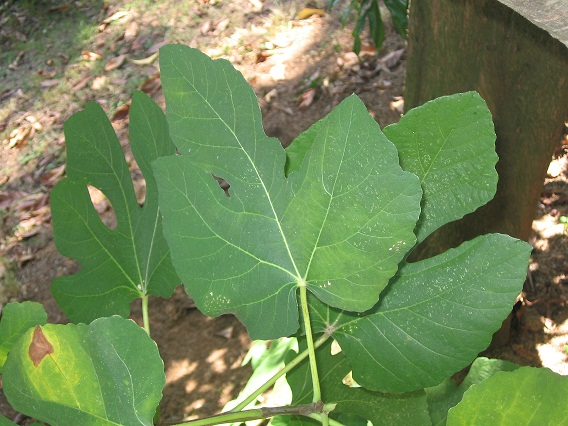
\includegraphics[width=100mm]{leaves.jpg}
	\caption{Caption of the image}
	\label{leave}
\end{center}
\end{figure}

\subsection{Handling bibliography}

Finally, let's find out how a nice bibliography is created. First, check the bibliography styles. A bibliography style tells the document how the references and the list of resources will look like. Currently there exists one style named "alphadin.bst".

In order to set the style do a \textbf{\textbackslash bibliographystyle\{alphadin\}} where "alphadin" (without the ending ".bst") sets the style. If you want to place the bibliography in your text then simply do \textbf{\textbackslash bibliography\{document\}}.

At the time you've created a bibliography (actually, it is created automatically when you create a new project) you can edit its entries by pressing the "Bibliography" button. You can come back here if you press it again. Now that you've entered all your books and articles in the bibliography simply do a \textbf{\textbackslash cite\{refname1\}} where "refname1" specifies the resource you want to cite.

A test: \cite{referenceName1} says that it is a good idea to use LaTeX.

% Create the bibliography right after the text
\bibliographystyle{alphadin}
\bibliography{document}

\end{document}
% All lines that begin with an '%' are comments and won't be displayed in the resulting document1main-branch222

% \documentclass{...} specifies the class of the document. The most common ones are 'book', 'report', 'article' and 'letter'
\documentclass{article}

% Allow the usage of umlauts and other non-ASCII characters
\usepackage[utf8]{inputenc}
% Allow the usage of graphics (.jpg, .png, etc.) in the document
\usepackage{graphicx}
% Allow the change of line spacing
\usepackage{setspace}

% Set line spacing to 1.5xxxneu
\onehalfspacing

% Start the document
\begin{document}

% Show the titlepage (see in 'Documents' below: titlepage.tex)
% Begin a new titlepage. Titlepages have special settings like the absence of page numbers.222
\begin{titlepage}

% Set the text of the page to right-aligned until \end{flushright}
\begin{flushright}

% Set the space between right page border and text to 2.5cm
\rightskip=-2.5cm

% Show an image at this position

\includegraphics[width=50mm]{logo_dark.png}

% Skip a little space
\bigskip
\bigskip
\bigskip
\bigskip

% Create a title for the document and write it in bold font
\LARGE{\textbf{Brief LaTeX Tutorial}}
% Again, do a line break
\linebreak
% Create a subtitle
\large{For LaTeX Beginners}

% Skip some space
\bigskip
\bigskip
\bigskip
\bigskip
\bigskip

% Write in very large letters
\LARGE{verbosus.com}
% Do a line break right after the \LARGE{...} text
\linebreak
% Write in large letters
\large{Free webservices and apps}

% Skip some space
\bigskip
\bigskip
\bigskip
\bigskip
\bigskip
\bigskip

\large{Documentation}

% Skip some space
\bigskip

\normalsize{Vienna, \the\month}

% Skip some space
\bigskip
\bigskip
\bigskip
\bigskip
\bigskip
\bigskip
\bigskip
\bigskip
\bigskip
\bigskip
\bigskip
\bigskip
\bigskip

% Provide some author information
\normalsize{Author:}
\linebreak
\large{Daniel Kuster, MSc}

% End right-alignment at this point
\end{flushright}
% End the title page
\end{titlepage}


% Create a new 1st level heading
\section{First level}

This is the text of the first chapter. If you want to create a subchapter then simply do \textbf{\textbackslash subsection\{Title of first subchapter\}}. If you want to move on to the next chapter then do \textbf{\textbackslash section\{Title of second chapter\}}.

% Create a new 2nd level heading
\subsection{Second level}

Here comes the text of the subsection of the first chapter. Now let's try to insert an image. Currently there exists one image with the name "leaves.jpg" which will be displayed at the current position. This can be changed by changing the [h] (stands for "here", place it at the current position if possible) to a [t] (stands for "top", place it at the beginning of a page if possible), [b] (stands for "bottom", place it at the bottom of a page if possible) or [p] (stands for "float page", place it on a separate page with other floating objects).

The image we've just inserted can be referenced by writing \textbf{\textbackslash ref\{leave\}}. As you can see the figure \ref{leave} shows some leaves.

\subsection{Handling other resource types}

There exist other very useful elements which can be inserted such as tables, itemized lists or description lists. You can try them by simply clicking on the small icons in the editor.

\begin{figure}[htp]
\begin{center}
	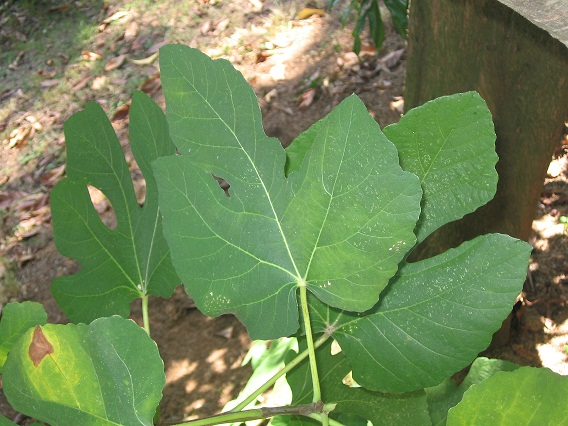
\includegraphics[width=100mm]{leaves.jpg}
	\caption{Caption of the image}
	\label{leave}
\end{center}
\end{figure}

\subsection{Handling bibliography}

Finally, let's find out how a nice bibliography is created. First, check the bibliography styles. A bibliography style tells the document how the references and the list of resources will look like. Currently there exists one style named "alphadin.bst".

In order to set the style do a \textbf{\textbackslash bibliographystyle\{alphadin\}} where "alphadin" (without the ending ".bst") sets the style. If you want to place the bibliography in your text then simply do \textbf{\textbackslash bibliography\{document\}}.

At the time you've created a bibliography (actually, it is created automatically when you create a new project) you can edit its entries by pressing the "Bibliography" button. You can come back here if you press it again. Now that you've entered all your books and articles in the bibliography simply do a \textbf{\textbackslash cite\{refname1\}} where "refname1" specifies the resource you want to cite.

A test: \cite{referenceName1} says that it is a good idea to use LaTeX.

% Create the bibliography right after the text
\bibliographystyle{alphadin}
\bibliography{document}

\end{document}
% All lines that begin with an '%' are comments and won't be displayed in the resulting document1main-branch222

% \documentclass{...} specifies the class of the document. The most common ones are 'book', 'report', 'article' and 'letter'
\documentclass{article}

% Allow the usage of umlauts and other non-ASCII characters
\usepackage[utf8]{inputenc}
% Allow the usage of graphics (.jpg, .png, etc.) in the document
\usepackage{graphicx}
% Allow the change of line spacing
\usepackage{setspace}

% Set line spacing to 1.5xxxneu
\onehalfspacing

% Start the document
\begin{document}

% Show the titlepage (see in 'Documents' below: titlepage.tex)
% Begin a new titlepage. Titlepages have special settings like the absence of page numbers.222
\begin{titlepage}

% Set the text of the page to right-aligned until \end{flushright}
\begin{flushright}

% Set the space between right page border and text to 2.5cm
\rightskip=-2.5cm

% Show an image at this position
\includegraphics[width=50mm]{logo_dark.png}

% Skip a little space
\bigskip
\bigskip
\bigskip
\bigskip

% Create a title for the document and write it in bold font
\LARGE{\textbf{Brief LaTeX Tutorial}}
% Again, do a line break
\linebreak
% Create a subtitle
\large{For LaTeX Beginners}

% Skip some space
\bigskip
\bigskip
\bigskip
\bigskip
\bigskip

% Write in very large letters
\LARGE{verbosus.com}
% Do a line break right after the \LARGE{...} text
\linebreak
% Write in large letters
\large{Free webservices and apps}

% Skip some space
\bigskip
\bigskip
\bigskip
\bigskip
\bigskip
\bigskip

\large{Documentation}

% Skip some space
\bigskip

\normalsize{Vienna, \the\month}

% Skip some space
\bigskip
\bigskip
\bigskip
\bigskip
\bigskip
\bigskip
\bigskip
\bigskip
\bigskip
\bigskip
\bigskip
\bigskip
\bigskip

% Provide some author information
\normalsize{Author:}
\linebreak
\large{Daniel Kuster, MSc}

% End right-alignment at this point
\end{flushright}
% End the title page
\end{titlepage}


% Create a new 1st level heading
\section{First level}

This is the text of the first chapter. If you want to create a subchapter then simply do \textbf{\textbackslash subsection\{Title of first subchapter\}}. If you want to move on to the next chapter then do \textbf{\textbackslash section\{Title of second chapter\}}.

% Create a new 2nd level heading
\subsection{Second level}

Here comes the text of the subsection of the first chapter. Now let's try to insert an image. Currently there exists one image with the name "leaves.jpg" which will be displayed at the current position. This can be changed by changing the [h] (stands for "here", place it at the current position if possible) to a [t] (stands for "top", place it at the beginning of a page if possible), [b] (stands for "bottom", place it at the bottom of a page if possible) or [p] (stands for "float page", place it on a separate page with other floating objects).

The image we've just inserted can be referenced by writing \textbf{\textbackslash ref\{leave\}}. As you can see the figure \ref{leave} shows some leaves.

\subsection{Handling other resource types}

There exist other very useful elements which can be inserted such as tables, itemized lists or description lists. You can try them by simply clicking on the small icons in the editor.

\begin{figure}[htp]
\begin{center}
	\includegraphics[width=100mm]{leaves.jpg}
	\caption{Caption of the image}
	\label{leave}
\end{center}
\end{figure}

\subsection{Handling bibliography}

\bibliographystyle{alphadin}
\bibliography{document}

\end{document}
